\documentclass[10pt,letterpaper]{article}

\usepackage[]{graphicx}\usepackage[]{color}
%% maxwidth is the original width if it is less than linewidth
%% otherwise use linewidth (to make sure the graphics do not exceed the margin)
\makeatletter
\def\maxwidth{ %
  \ifdim\Gin@nat@width>\linewidth
    \linewidth
  \else
    \Gin@nat@width
  \fi
}
\makeatother

\definecolor{fgcolor}{rgb}{0.345, 0.345, 0.345}
\newcommand{\hlnum}[1]{\textcolor[rgb]{0.686,0.059,0.569}{#1}}%
\newcommand{\hlstr}[1]{\textcolor[rgb]{0.192,0.494,0.8}{#1}}%
\newcommand{\hlcom}[1]{\textcolor[rgb]{0.678,0.584,0.686}{\textit{#1}}}%
\newcommand{\hlopt}[1]{\textcolor[rgb]{0,0,0}{#1}}%
\newcommand{\hlstd}[1]{\textcolor[rgb]{0.345,0.345,0.345}{#1}}%
\newcommand{\hlkwa}[1]{\textcolor[rgb]{0.161,0.373,0.58}{\textbf{#1}}}%
\newcommand{\hlkwb}[1]{\textcolor[rgb]{0.69,0.353,0.396}{#1}}%
\newcommand{\hlkwc}[1]{\textcolor[rgb]{0.333,0.667,0.333}{#1}}%
\newcommand{\hlkwd}[1]{\textcolor[rgb]{0.737,0.353,0.396}{\textbf{#1}}}%
\let\hlipl\hlkwb

\usepackage{framed}
\makeatletter
\newenvironment{kframe}{%
 \def\at@end@of@kframe{}%
 \ifinner\ifhmode%
  \def\at@end@of@kframe{\end{minipage}}%
  \begin{minipage}{\columnwidth}%
 \fi\fi%
 \def\FrameCommand##1{\hskip\@totalleftmargin \hskip-\fboxsep
 \colorbox{shadecolor}{##1}\hskip-\fboxsep
     % There is no \\@totalrightmargin, so:
     \hskip-\linewidth \hskip-\@totalleftmargin \hskip\columnwidth}%
 \MakeFramed {\advance\hsize-\width
   \@totalleftmargin\z@ \linewidth\hsize
   \@setminipage}}%
 {\par\unskip\endMakeFramed%
 \at@end@of@kframe}
\makeatother

\definecolor{shadecolor}{rgb}{.97, .97, .97}
\definecolor{messagecolor}{rgb}{0, 0, 0}
\definecolor{warningcolor}{rgb}{1, 0, 1}
\definecolor{errorcolor}{rgb}{1, 0, 0}
\newenvironment{knitrout}{}{} % an empty environment to be redefined in TeX

\usepackage{alltt}
\usepackage[top=0.85in,left=1.75in,footskip=0.75in]{geometry}

% amsmath and amssymb packages, useful for mathematical formulas and symbols
\usepackage{amsmath,amssymb}

% Use adjustwidth environment to exceed column width (see example table in text)
\usepackage{changepage}

% Use Unicode characters when possible
\usepackage[utf8x]{inputenc}

% textcomp package and marvosym package for additional characters
\usepackage{textcomp,marvosym}

% cite package, to clean up citations in the main text. Do not remove.
\usepackage{cite}

% Use nameref to cite supporting information files (see Supporting Information section for more info)
\usepackage{nameref,hyperref}

% line numbers
\usepackage[right]{lineno}

% ligatures disabled
\usepackage{microtype}
\DisableLigatures[f]{encoding = *, family = * }

% color can be used to apply background shading to table cells only
\usepackage[table]{xcolor}

% array package and thick rules for tables
\usepackage{array}

% bold math symbols package
\usepackage{bm}

% nice figures and captions
\usepackage{graphicx}

% diagrams or complicated equations
\usepackage{tikz}

% vertical and horizontal dashed lines
\usepackage{arydshln}

%\usepackage{floatflt}
%\usepackage{nonfloat}
\usepackage{float}
\usepackage{wrapfig}

\usepackage{harpoon}
\usepackage{fdsymbol}

\usepackage{longtable,booktabs}
\usepackage{tabu}

%\renewcommand{\arraystretch}{1.2}
%\setlength{\tabcolsep}{12pt}

% create "+" rule type for thick vertical lines
\newcolumntype{+}{!{\vrule width 2pt}}

% create \thickcline for thick horizontal lines of variable length
\newlength\savedwidth
\newcommand\thickcline[1]{%
  \noalign{\global\savedwidth\arrayrulewidth\global\arrayrulewidth 2pt}%
  \cline{#1}%
  \noalign{\vskip\arrayrulewidth}%
  \noalign{\global\arrayrulewidth\savedwidth}%
}

% \thickhline command for thick horizontal lines that span the table
\newcommand\thickhline{\noalign{\global\savedwidth\arrayrulewidth\global\arrayrulewidth 2pt}%
\hline
\noalign{\global\arrayrulewidth\savedwidth}}


% Remove comment for double spacing
%\usepackage{setspace} 
%\doublespacing

% Text layout
% \raggedright
\setlength{\parindent}{0.5cm}
\textwidth 5.25in 
\textheight 8.75in

% Bold the 'Figure #' in the caption and separate it from the title/caption with a period
% Captions will be left justified
\usepackage[aboveskip=1pt,labelfont=bf,labelsep=period,justification=raggedright,singlelinecheck=off]{caption}
\renewcommand{\figurename}{Fig}

% Use the PLoS provided BiBTeX style
%\bibliographystyle{plos2015}


% Remove brackets from numbering in List of References
\makeatletter
\renewcommand{\@biblabel}[1]{\quad#1.}
\makeatother

% define theorem and definition environments commands
\newtheorem{theorem}{Theorem}[section]
\newtheorem{definition}{Definition}[section]

% Header and Footer with logo
\usepackage{lastpage,fancyhdr,graphicx}
\usepackage{epstopdf}
%\pagestyle{myheadings}
\pagestyle{fancy}
\fancyhf{}
%\setlength{\headheight}{27.023pt}
%\lhead{\includegraphics[width=2.0in]{PLOS-submission.eps}}
\rfoot{\thepage/\pageref{LastPage}}
\renewcommand{\headrulewidth}{0pt}
\renewcommand{\footrule}{\hrule height 2pt \vspace{2mm}}
\fancyheadoffset[L]{2.25in}
% \fancyfootoffset[L]{1.25in}
\lfoot{\today}


\restylefloat{figure}


%% Include all macros below

\newcommand{\lorem}{{\bf LOREM}}
\newcommand{\ipsum}{{\bf IPSUM}}

\def\lf{\left\lfloor}   
\def\rf{\right\rfloor}

\def\ri{R_i}
\def\rj{R_j}
\def\kmi{k_{M_i}}
\def\khi{k_{H_i}}
\def\hji{H_{j_i}}
\def\ma{\overline{M}_a}
\def\ha{\overline{H}_a}
\def\mnu{M_\nu}
\def\hnu{H_\nu}
\def\myd{\text{diff}}
\def\ka{\bar{k}_\alpha}
\def\mji{M_{j_i}}

%% END MACROS SECTION
\IfFileExists{upquote.sty}{\usepackage{upquote}}{}
\begin{document}
\vspace*{0.2in}

% Title must be 250 characters or less.
% \begin{flushleft}
{\Large
\textbf\newline{Blessings of Dimensionality: Finding the optimal k for nearest-neighbor projected-distance feature selection (for detecting interaction and main effects in high dimensional data)} % Please use "sentence case" for title and headings (capitalize only the first word in a title (or heading), the first word in a subtitle (or subheading), and any proper nouns).
}
%\newline
% Insert author names, affiliations and corresponding author email (do not include titles, positions, or degrees).
\begin{center}
  \begin{tabular}{l}
  Bryan A. Dawkins$^{\text{1}}$, Trang T. Le$^{\text{2}}$ and Brett A. McKinney$^{\text{1,3,}*}$ \\
  $^{\text{1}}$Department of Mathematics, University of Tulsa, Tulsa, OK 74104, USA \\
  $^{\text{2}}$Department of Biostatistics, Epidemiology and Informatics, University of \\
  \hphantom{2}Pennsylvania, Philadelphia, PA 19104 \\
  $^{\text{3}}$Tandy School of Computer Science, University of Tulsa, Tulsa, OK 74104, USA. \\
  $*$Correspondence: brett.mckinney@gmail.com
  \end{tabular}
\end{center}


% \end{flushleft}
% Please keep the abstract below 300 words
\section*{Abstract}
It is commonly known that high-throughput data has many inherent statistical challenges, such as multiple testing, sparsity and over fitting. Collectively, these challenges are known as the Curse of Dimensionality. Here we highlight an important Blessing of Dimensionality: the ability to identify interactions and main effects with neighborhoods of instances. We review the nearest-neighbor concept for finding interactions among attributes. We present a novel simulation method for generating data with both main effects and interactions from random networks with fine-tuned control over interaction effect size. Using our new simulation strategy, we determine optimal fixed $k$ for neighborhood computation in nearest-neighbor distance-based feature selection for different ratios of main/interaction effect among functional attributes and different combinations of main and interaction effect sizes. We discuss ways to maximize the blessings and minimize the curses of dimensionality to reliably identify interactions and main effects. Our results will show how optimal fixed $k$ changes under a variety of conditions that we see in real data, which will serve as a guide for other researchers using nearest-neighbor distance-based feature selection. 

\linenumbers

\section*{Introduction}

Relief-based methods identify interacting attributes as important by using nearest-neighbor information in higher dimensions (the ``blessings of dimensionality''). Myopic methods that do not account for information from higher dimensions such as univariate tests are susceptible to false negatives when there are interactions. For example, in the plot of variable A versus C in a three-variable simulation (Figure~\ref{fig:ABC}-I), variable A appears to show no difference between cases and controls (the marginal group means are the same). However, A is actually simulated to have a strong differential correlation with B, conditioned on the outcome variable (Figure~\ref{fig:ABC}-II). Current Relief-based methods determine the importance of an attribute by computing the average difference of attribute $A$ value between a target instance (X) and its nearest instance from the opposite class (Miss), $d_{\text{X,M}}(A)$, subtracted from the similarly projected difference of target X and its nearest instance from the same class (Hit), $d_{\text{X,H}}(A)$. A positive value from this calculation, i.e., $d_{\text{X,M}}(A)-d_{\text{X,H}}(A) > 0$, suggests that attribute A is useful for discriminating between cases and controls.  

\begin{figure}[H]
	\centering
	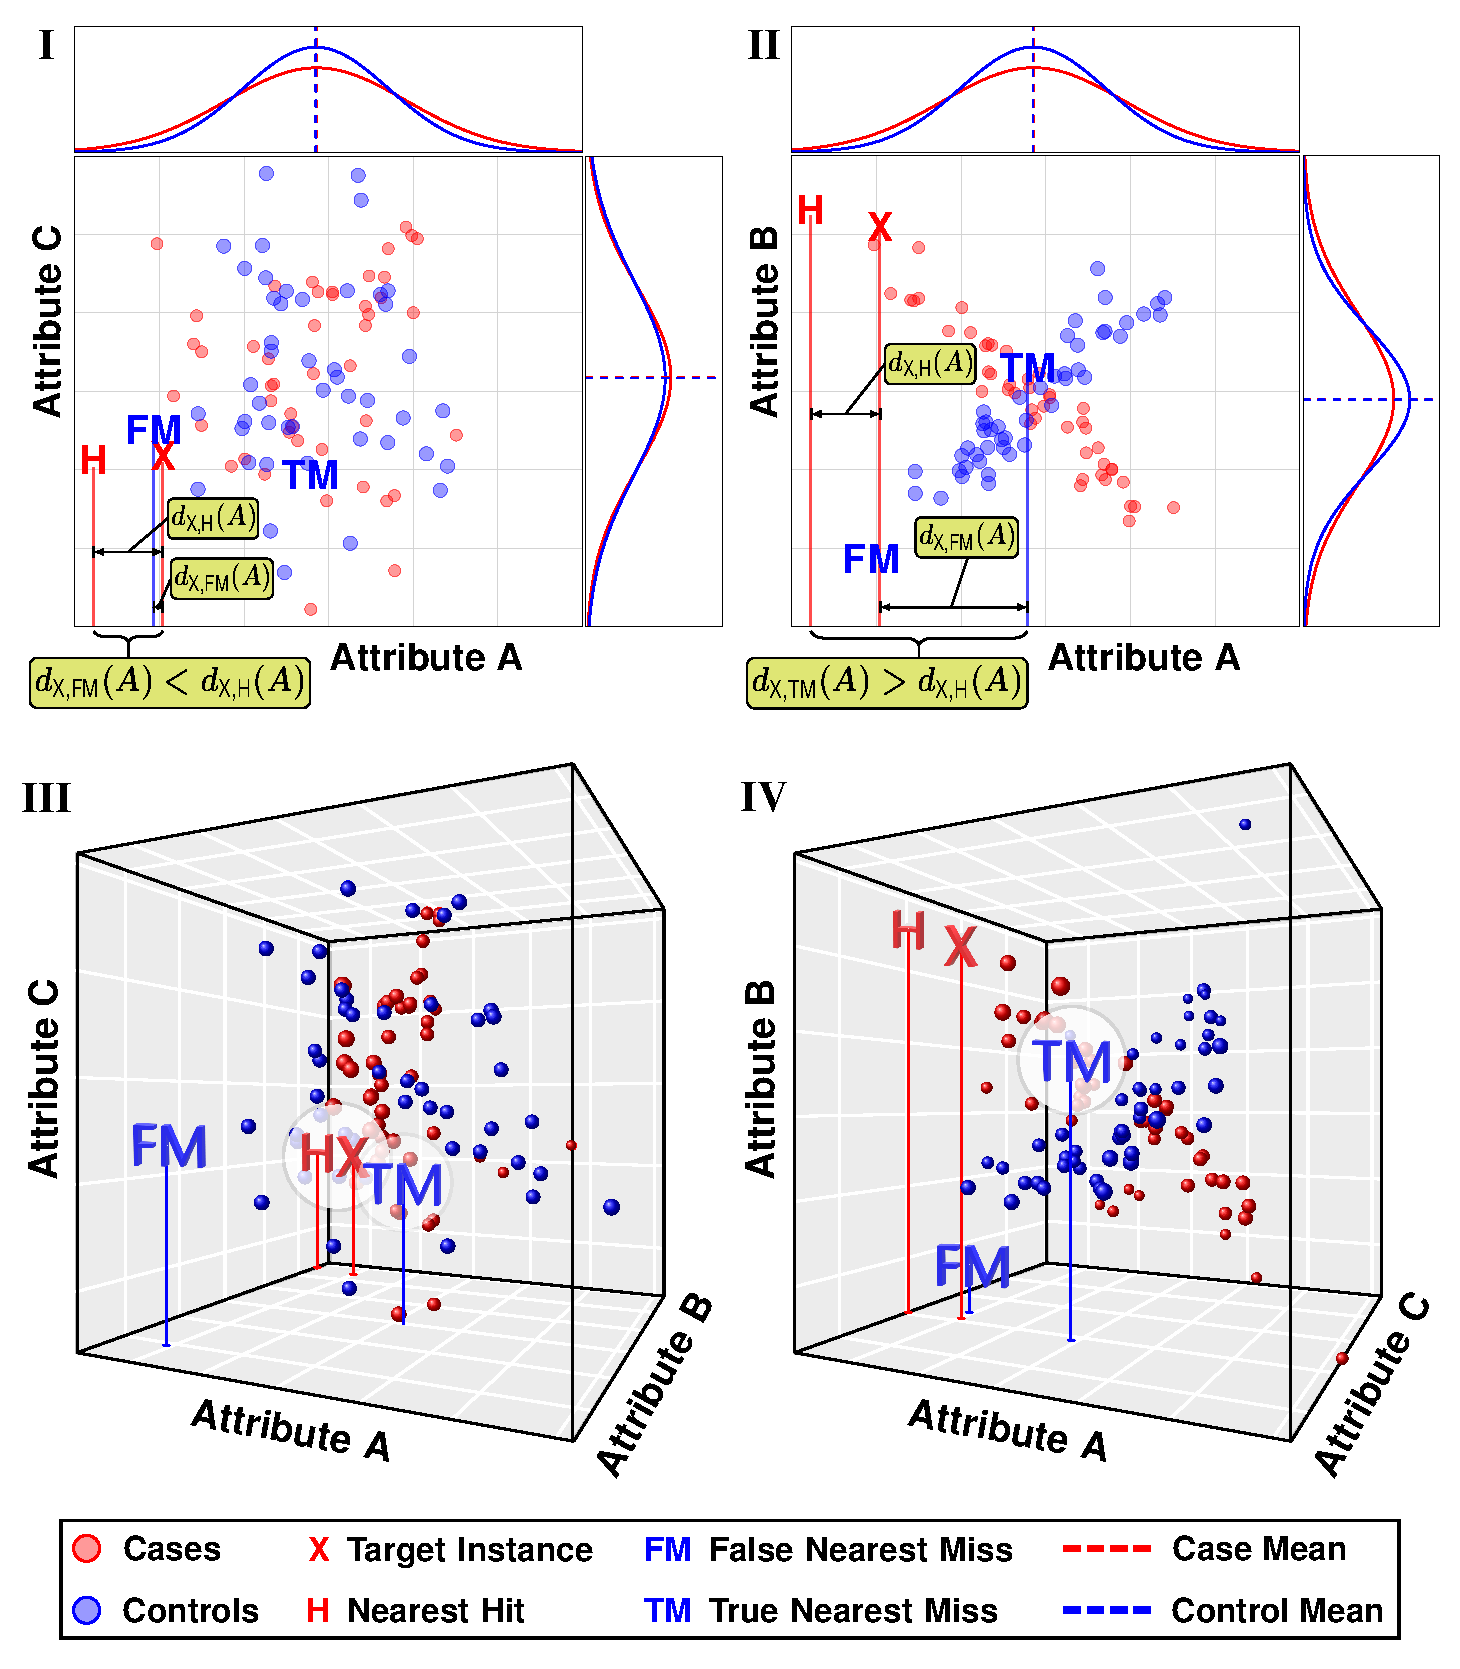
\includegraphics[width=\textwidth]{2by2_arrangementABC.pdf}
	\caption{{\bf Imposters vs true neighbors in the presence of interactions with three variables}. Attributes A, B, and C have no main effect. (\textbf{\fontfamily{ptm}\selectfont I}) Scatter plot of simulated irrelevant Attribute C with a functional Attribute A. (\textbf{\fontfamily{ptm}\selectfont II}) Scatter plot of Attributes A and B, which interact through differential correlation. Computing nearest neighbors with irrelevant attributes (\textbf{\fontfamily{ptm}\selectfont I}) or lower dimensions leads to imposter nearest neighbors and degrades the ability of Relief-based methods to identify interaction effects. Computing distances in only these two dimensions leads to an imposter false miss (FM) for the nearest neighbor from the opposite outcome class for target instance X. This imposter leads to Attribute A predicting closer projected distances for misses than hits (H), which incorrectly indicates that A is a poor discriminator (yellow boxes in \textbf{\fontfamily{ptm}\selectfont I}). (\textbf{\fontfamily{ptm}\selectfont III-IV}) Computing nearest neighbors in higher dimensions or with the correct interaction partner leads to imposter nearest neighbor (FM) being replaced by the true nearest miss neighbor (TM) for target instance X, which correctly leads to Attribute A predicting closer projected distances for hits (H) than misses, which is an indication that Attribute A is a good discriminator (yellow boxes \textbf{\fontfamily{ptm}\selectfont II}).}\label{fig:ABC}
\end{figure}
%\begin{figure}[h!]
%%\begin{center}
%\begin{minipage}[c]{0.4\textheight}
%\centering
%		\framebox{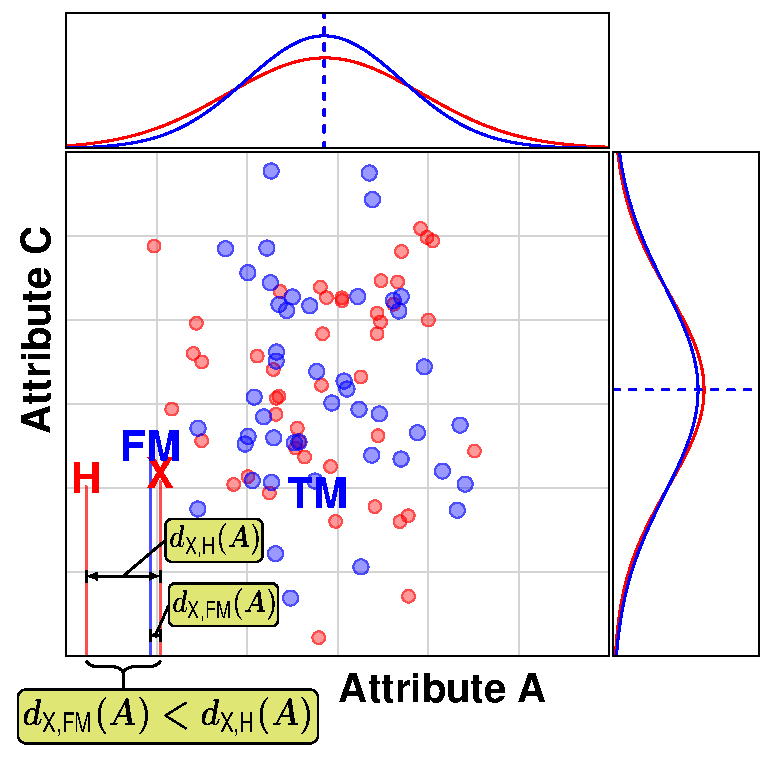
\includegraphics[width=0.8\textwidth]{glmSTIR_figure_2D_final_CvsA.pdf}}
%\end{minipage} \hspace{-0.4cm}
%\begin{minipage}[c]{0.5\textwidth}
%\centering
%\caption{{\bf Imposters vs true neighbors in the presence of interactions with three variables}. Scatter plot of simulated irrelevant Attribute C with a functional Attribute A {\bf(a)}. None of the attributes has a main effect, but Attribute B and C interact through differential correlation {\bf(b)}. Computing nearest neighbors with irrelevant attributes {\bf(a)} or lower dimensions leads to imposter nearest neighbors and degrades the ability of Relief-based methods to identify interaction effects. Computing distances in only these two dimensions leads to an imposter false miss (FM) for the nearest neighbor from the opposite outcome class for target instance X. This imposter leads to attribute A predicting closer projected distances for misses than hits (H), which incorrectly indicates that A is a poor discriminator (yellow boxes in {\bf a}). Computing nearest neighbors in higher dimensions {\bf(c-d)} or with the correct interaction partner leads to imposter nearest neighbor (FM) being replaced by the true nearest miss neighbor (TM) for target instance X, which correctly leads to attribute A predicting closer projected distances for hits (H) than misses, which is an indication that attribute A is a good discriminator (yellow boxes {\bf(b)}).}\label{fig:2dAvC}
%\end{minipage}
%%\end{center}
%\end{figure}

%\newpage

%\begin{figure}[ht!]
%\begin{wrapfigure}{l}{0.6\textwidth}
%    \vspace{-12pt}
%	\centering
%	\framebox{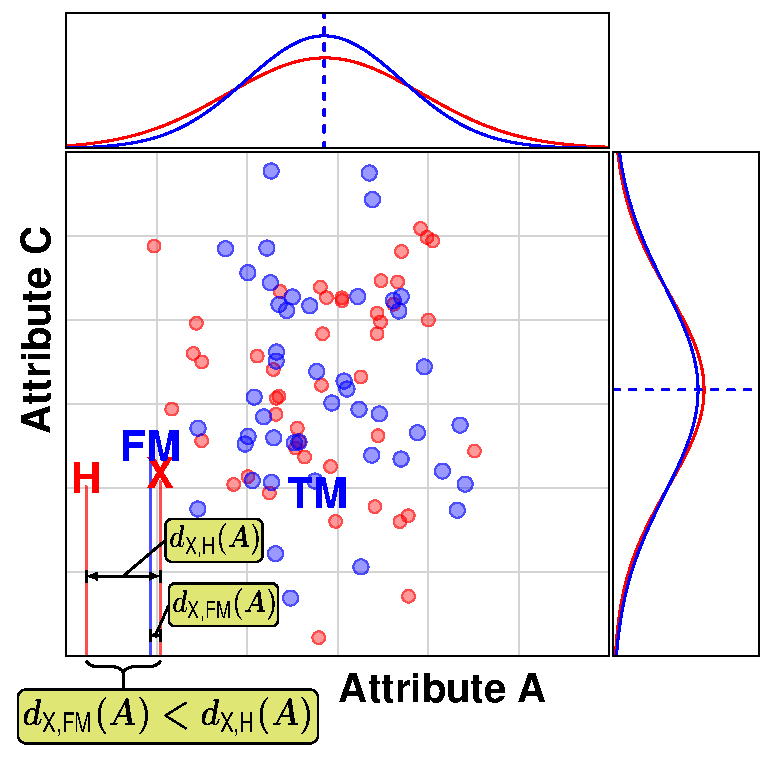
\includegraphics[width=0.55\textwidth]{glmSTIR_figure_2D_final_CvsA.pdf}}
%\end{wrapfigure}
%\noindent\refstepcounter{figure}\textbf{Fig \thefigure \label{fig:2dAvC}.} \textbf{Imposters vs true neighbors in the presence of interactions with three variables}. Scatter plot of simulated irrelevant Attribute C with a functional Attribute A \textbf{(a)}. None of the attributes has a main effect, but Attribute B and C interact through differential correlation \textbf{(b)}. Computing nearest neighbors with irrelevant attributes \textbf{(a)} or lower dimensions leads to imposter nearest neighbors and degrades the ability of Relief-based methods to identify interaction effects. Computing distances in only these two dimensions leads to an imposter false miss (FM) for the nearest neighbor from the opposite outcome class for target instance X. This imposter leads to attribute A predicting closer projected distances for misses than hits (H), which incorrectly indicates that A is a poor discriminator (yellow boxes in \textbf{(a)}). Computing nearest neighbors in higher dimensions \textbf{(c-d)} or with the correct interaction partner leads to imposter nearest neighbor (FM) being replaced by the true nearest miss neighbor (TM) for target instance X, which correctly leads to attribute A predicting closer projected distances for hits (H) than misses, which is an indication that attribute A is a good discriminator (yellow boxes \textbf{(b)}).
%\end{figure}

Relief-based methods use information from all available attributes (omnigenic) to estimate an attribute's importance. However, if relevant higher-dimensional information is not used to establish the neighborhoods of instances, these methods will miss the effect of A because ``imposter'' neighbors will be used in the attribute estimate (False Miss (FM) in Fig.~\ref{fig:ABC}-I, where $d_{\text{X,FM}}(A)<d_{\text{X,H}}(A)$).  If one were to compute nearest neighbors in the A-C plane (ignoring the B dimension), the nearest miss would be an imposter (FM), which leads to a negative contribution to the importance score for A. One might call this C attribute a type-I confounding attribute because it increases the chances of interacting attributes to be false negatives. When nearest neighbors are calculated based on higher dimensions with relevant information (Fig.~\ref{fig:ABC}-III), it is clear that TM is closer to X than FM. The imposter (FM) is replaced by the true nearest miss (TM) and attribute A correctly shows a greater projected difference between misses than hits (Fig.~\ref{fig:ABC}-II $d_{\text{X,TM}}(A)>d_{\text{X,H}}(A)$), which is the signature of an important attribute. Univariate methods still cannot find the importance of A unless the interaction is explicitly modeled, but as long as functional variables A and B are in the space for nearest neighbor calculations (Fig.~\ref{fig:ABC}-III - IV), imposters can be excluded and Relief-based methods will find that A (and B) are important discriminators. 

%\begin{figure}[ht!]
%%\begin{center}
%\begin{minipage}[c]{0.4\textheight}
%\centering 
%		\framebox{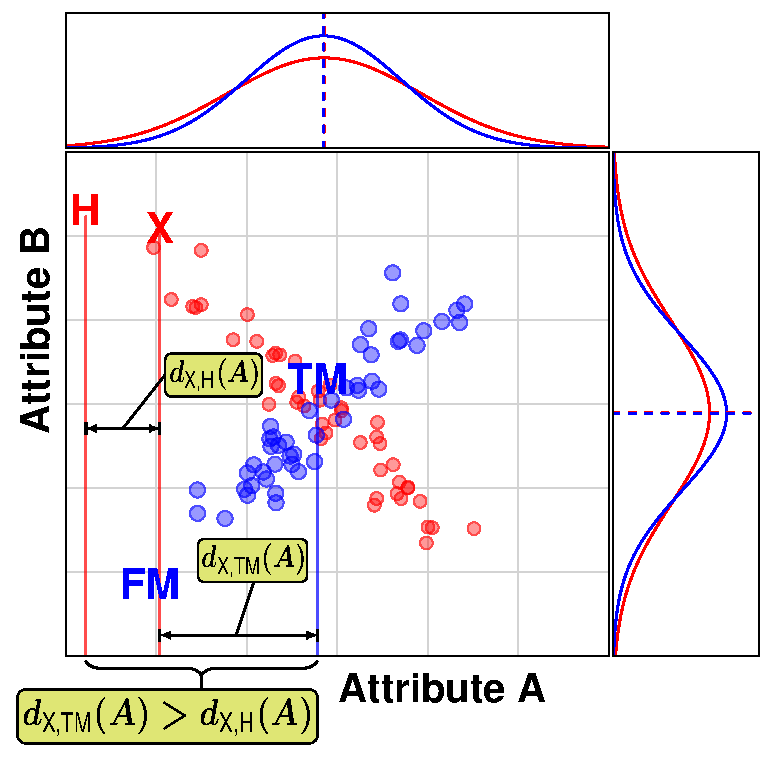
\includegraphics[width=0.8\textwidth]{glmSTIR_figure_2D_final_BvsA.pdf}}
%\end{minipage} \hspace{-0.4cm}
%\begin{minipage}[c]{0.5\textwidth}
%\centering
%\caption{{\bf True neighbors}}\label{fig:2dAvB}
%\end{minipage}
%%\end{center}
%\end{figure}  

%\begin{figure}[ht!]
%%\begin{center}
%\begin{minipage}[c]{0.4\textheight}
%\centering
%		\framebox{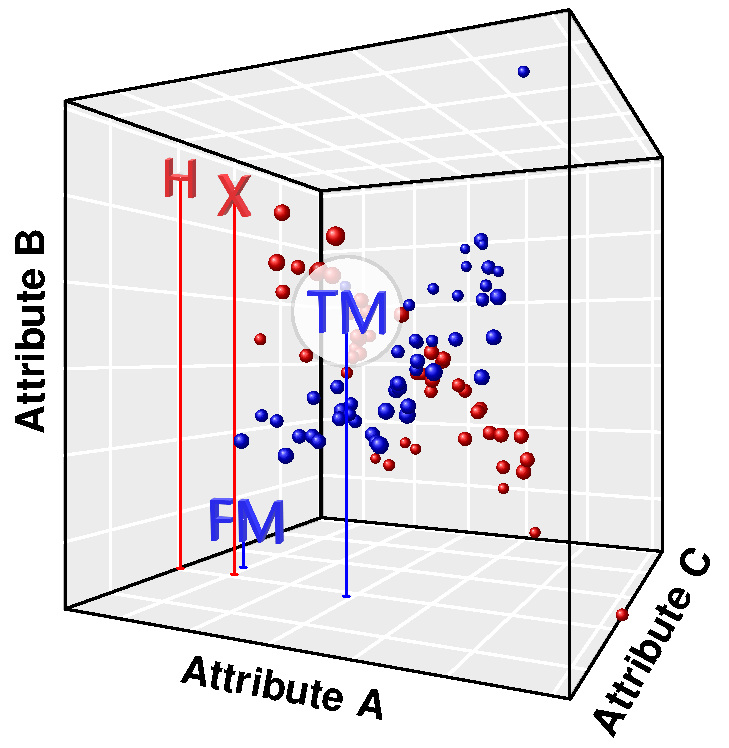
\includegraphics[width=0.8\textwidth]{nice_box_2D_points.pdf}}
%\end{minipage} \hspace{-0.4cm}
%\begin{minipage}[c]{0.5\textwidth}
%\centering
%\caption{{\bf 3D AB view}. Still working on this. }\label{fig:3d_c}
%\end{minipage}
%%\end{center}
%\end{figure}  

%\begin{figure}[ht!]
%%\begin{center}
%%\begin{minipage}[c]{0.4\textheight}
%\centering
%		\framebox{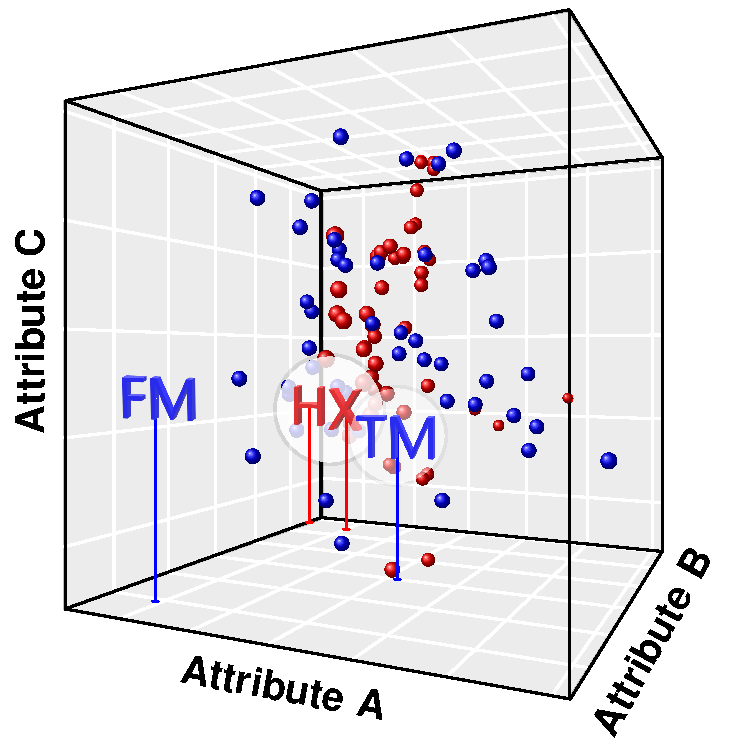
\includegraphics[width=0.8\textwidth]{nice_box_2D_points2.pdf}}
%\end{minipage} \hspace{-0.4cm}
%\begin{minipage}[c]{0.5\textwidth}
%\centering
%\caption{{\bf 3D AC view}. Still working on this. }\label{fig:3d_d}
%\end{minipage}
%%\end{center}
%\end{figure}  

%Using same interaction, increase background noise genes to see degrading of A and B Relief importance because of curse of dimensionality (sparseness). 

\begin{figure}[H]
	\centering
	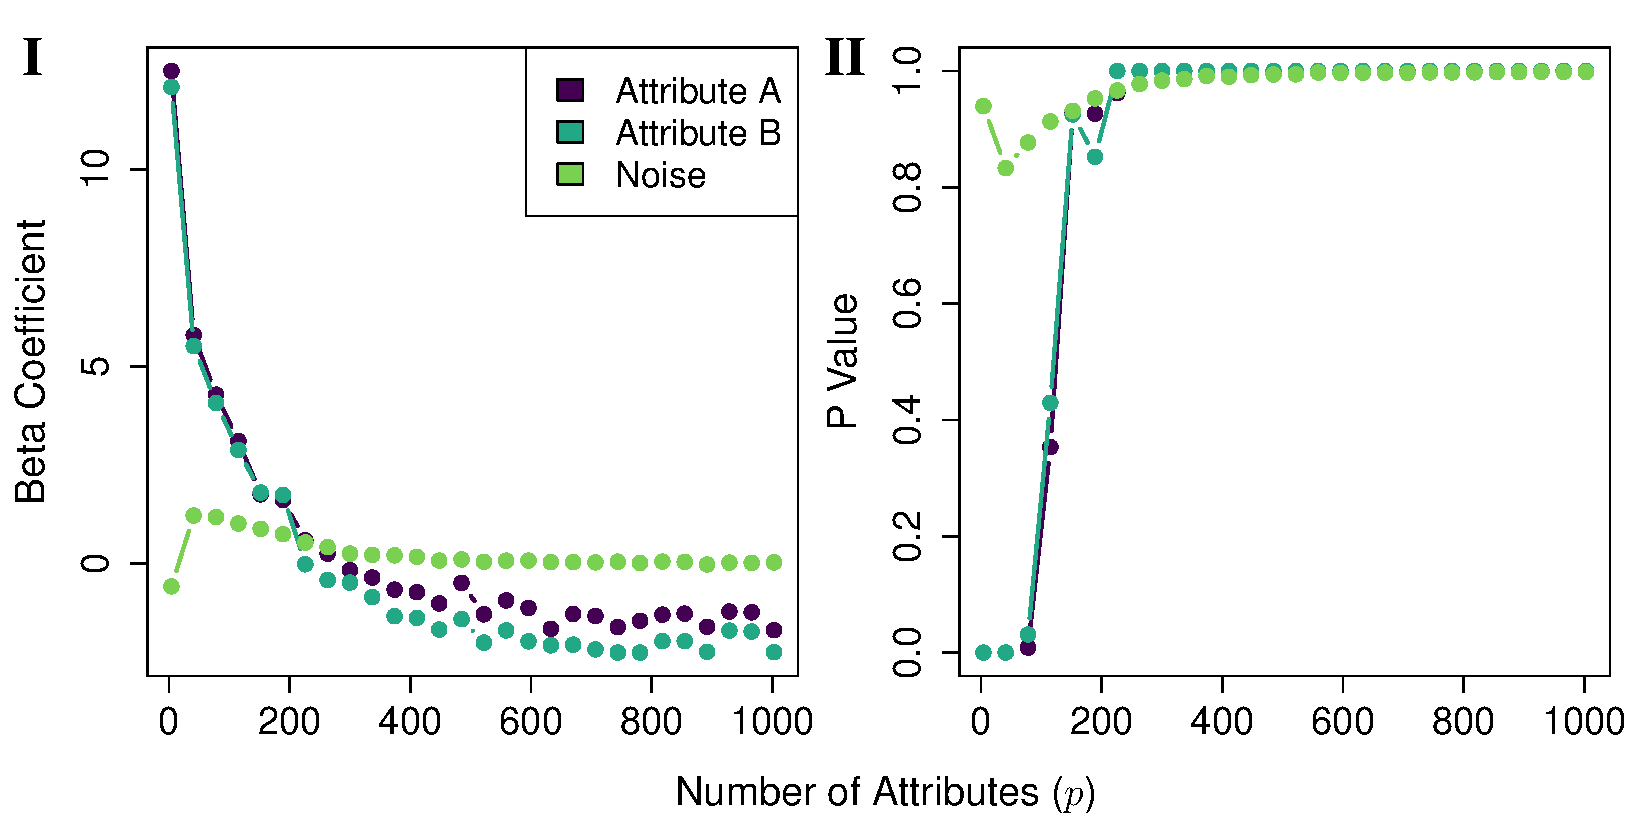
\includegraphics[width=1\textwidth]{betas_and_pvals_vs_p_ABC.pdf}
	\caption{Interacting features A and B in the presence of noise. (\textbf{I}) Standardized beta coefficients of interacting features A and B and irrelevant features plotted vs the total number of features $p$. As more irrelevant features are added to the simulated interacting features A and B, beta coefficients decrease quickly. At about 200 features (198 irrelevant), A and B have beta coefficients close to 0. (\textbf{II}) P values corresponding to standardized beta coefficients of interacting features A and B and irrelevant features plotted vs the total number of features $p$. As more irrelevant features are added, P values quickly approach 1.}\label{fig:ABC_plus_noise}
\end{figure}


Using the same interaction partners (A and B), we explored the effects of increasing the level of noise (sparsity) in the data (Figure~\ref{fig:ABC_plus_noise}). We iteratively added random null standard normal features and computed standardized beta coefficients (Figure~\ref{fig:ABC_plus_noise}-I) and corresponding pseudo P values (Figure~\ref{fig:ABC_plus_noise}-II) using a new method called Nearest-neighbor Projected Distance Regression (NPDR)~\cite{npdr2}. For binary response variables, like case-control outcomes, NPDR computes a standardized beta coefficient for a generalized linear model (GLM) (Figure~\ref{fig:npdr_finished}). The argument to the logit function is $\text{p}^\text{miss}_{ij}$, which is the probability that instances $i,j$ are in different phenotype classes. This argument models the binary outcome diff, which is given by the following
%
\begin{equation}\label{eq:diff_outcome}
\text{d}^\text{miss}_{ij}(\overrightharpoon{y})=\begin{cases}
0 & y_i = y_j, \\
1 & \text{else}.
\end{cases}
\end{equation} 

For each value of $p$, we generated 10 separate sets of irrelevant attributes, combined them with attributes A and B, and computed beta coefficients and P values. After all 10 iterations for a fixed value of $p$, we took the average of the beta coefficients (Figure~\ref{fig:ABC_plus_noise}-I) and the average of the corresponding pseudo P values (Figure~\ref{fig:ABC_plus_noise}-II). As functionality becomes more sparse with respect to all features, it becomes increasingly difficult to detect interacting partners A and B. In fact, the beta coefficients are approximately zero when there are approximately 200 features in this simulated data. By chance, there are many irrelevant attributes that have larger beta coefficients than A and B. 

\begin{figure}[h!]
	\centering
	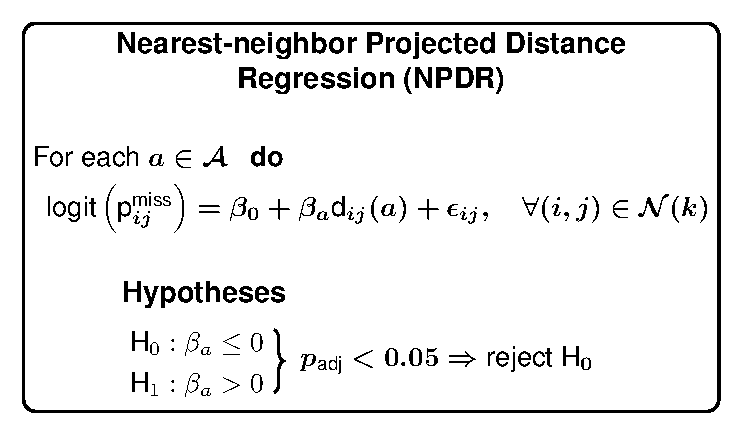
\includegraphics[width=0.85\textwidth]{npdr_finished_diagram.pdf}
	\caption{Nearest-neighbor Projected Distance Regression for binary response (case-control)~\cite{npdr2}. For each attribute $a \in \mathcal{A}$, where $\mathcal{A}$ is the collection of all attributes, we compute standardized beta coefficients for a generalized linear model, where the predictors ($\text{d}_{ij}(a) = |X_{ia} - X_{ja}|$) are one-dimensional projected distances (diffs) with respect to a particular attribute ($a$). The argument $\text{p}^\text{miss}_{ij}$ is the probability that instances ($i,j$) are in different phenotype classes. The logit function models the binary hit-miss phenotype projection (Eq.~\ref{eq:diff_outcome}). Significant adjusted pseudo P values ($p_\text{adj}$) lead to the rejection of the null hypothesis $\beta_a \leq 0$. The set $\mathcal{N}(k)$ is the collection of all neighbor ordered pairs such that each target instances neighborhood has exactly $k$ nearest neighbors.}\label{fig:npdr_finished}
\end{figure}

\section{Neighborhood methods}
Nearest-neighbor projected distance (NPD) methods rely on a neighborhood algorithm for feature selection. One may specify a fixed $k$ number of neighbors, a fixed radius, an average radius SURF, a MultiSURF radius that adapts for each instance~\cite{urbanowicz17}, or a variable-wise optimized $k$~\cite{mckinney13}. The definitive difference between fixed $k$ and either fixed or adaptive radius methods is that there is always a deterministic number of neighbors in fixed $k$ neighborhoods, but there is a variable neighborhood order in each fixed or adaptive radius method. In nearest-neighbor feature selection, neighborhood order is directly related to selected feature quality. Correlation and interaction effects change the distribution of pairwise distances between instances, which can change the probability of neighborhood inclusion for fixed or adaptive radius methods. In order to select the best set of features from data, it is important to know how pairwise feature correlation changes the optimal neighborhood order. We approach this problem by first determining the functional relationship between fixed $k$ and MultiSURF radius in data with negligible pairwise feature correlation and no effects.

\section{Derivation of expected \texorpdfstring{$k$}{} for MultiSURF neighborhoods}\label{sec:expected-k}
The MultiSURF radius for an instance is the mean of its distances to all other instances subtracted by $\alpha=1/2$ of the standard deviation of this mean. Previously we showed empirically for balanced case-control datasets that a good constant $k$ approximation to the expected number of neighbors within the multiSURF radii is $k=m/6$~\cite{stir}, where $m$ is the number of samples. Here we derive a more exact theoretical mean that shows the mathematical connection between neighbor-finding methods. This fixed $k$ approximation to MultiSURF is independent of the type of data and the particular radii of each instance in the data.

The distance between instances ($i,j \in \mathcal{I}$, $|\mathcal{I}|=m$) in the data set $X^{m \times p}$ of $m$ instances and $p$ attributes is calculated in the space of all attributes ($a \in \mathcal{A}$, $|\mathcal{A}|=p$) using a metric such as
\begin{equation}\label{eq:D}
% D^{(q)}_{ij}=\left(\sum_{a\in A}|\text{d}^{\text{type}}_{ij}(a)|^q\right)^{1/q},
D^{(q)}_{ij}=\left(\sum_{a\in \mathcal{A}}|\text{d}_{ij}(a)|^q\right)^{1/q},
\end{equation}
%
which is typically Manhattan ($q=1$) but may also be Euclidean ($q=2$). The quantity 
$\text{d}_{ij}(a)$,
known as a ``$\text{diff}$'' in Relief literature, is the projection of the distance between instances $i$ and $j$ onto the attribute $a$ dimension. The 
% ``type'' refers to the data type of the attribute
function $\text{d}_{ij}(a)$ supports any type of attributes
(e.g., numeric and categorical).
For example, the projected difference between two instances $i$ and $j$ for a continuous numeric ($\text{d}^{\text{num}}$) attribute $a$ may be
%\begin{equation}\label{eq:diff}
%\text{diff}^{(\text{num})}(a,(\ri,\rj))=\frac{|\text{value}(a,\ri)-\text{value}(a,\rj)%|}{\max(a)-\min(a)}.
%\end{equation}
\begin{equation}\label{eq:diff}
\begin{aligned}
\text{d}^{\text{num}}_{ij}(a)&=\text{diff}(a,(i,j))\\
                                            & = {|\hat{X}_{ia}-\hat{X}_{ja}|},
\end{aligned}
\end{equation}
where $\hat{X}$ represents the standardized data matrix $X$.
We use a simplified d$_{ij}(a)$ notation in place of the $\text{diff}(a,(i,j))$ notation that is customary in Relief-based methods.
NPDR omits the division by $\max(a)-\min(a)$ used by Relief to constrain scores to the interval from $-1$ to $1$ because NPDR scores are standardized regression coefficients with corresponding P values, so any scaling operation at this stage is unnecessary for comparing attribute scores. 
%\emph{Omit: The scaling may alleviate bias in the distance calculation. However, standardizing the data matrix $X$ ($\hat{X}$) should have the same effect without division by $\max(a)-\min(a)$, which has usual distribution properties for distances (expand).}
The numeric d$^{\text{num}}_{ij}(a)$ projection is simply the absolute difference between row elements $i$ and $j$ of the data matrix $X^{m \times p}$ for the attribute column $a$. 

The NPDR neighborhood set $\mathcal{N}$ of ordered pair indices is defined as follows. Instance $i$ is a point in $p$ dimensions, and we designate the topological neighborhood of $i$ as $N_{i}$. This neighborhood is a set of other instances trained on the data $X^{m \times p}$ and depends on the type of Relief neighborhood method (e.g., fixed $k$ or adaptive radius) and the type of metric (e.g., Manhattan or Euclidean). If instance $j$ is in the neighborhood of $i$ ($j \in N_{i}$), then the ordered pair $(i,j) \in \mathcal{N}$ for the projected-distance regression analysis. The ordered pairs constituting the neighborhood can then be represented as nested sets:
\begin{equation}\label{eq:N}
\mathcal{N}=\{\{(i, j)\}_{i=1}^{m}\}_{\{j \ne i : j \in N_{i}\}}.
\end{equation}
The cardinality of the set $\{j \ne i : j \in N_{i}\}$ is $k_i$, the number of nearest neighbors for subject $i$. For fixed $k$, this cardinality is just $k_i = k$ for each target instance $i \in \mathcal{I}$.

\subsection{Predicted number of neighbors in the MultiSURF \texorpdfstring{$\alpha$}{} neighborhood}

Regardless of the predictor data type (numeric or categorical), the distribution of the $p$ predictors (uniform, Gaussian, or binomial), or the metric used to compute distances (Manhattan or Euclidean), the $m(m-1)/2$ pairwise distances in the $p$-dimensional space are well approximated by a normal distribution. An instance $j$ is in the adaptive $\alpha$-radius neighborhood of $i$ ($j \in N^{\alpha}_{i}$) under the condition
%\begin{equation}
%\bar{D = \frac{2p}{\sqrt{\pi}}
%\end{equation}
%
%\begin{equation}
%\sigma_{D} = \frac{2p(\pi-2)}{\pi}
%\end{equation}
%
\begin{equation}
D_{ij} \le \, R_i^{\alpha} \implies j \in N^{\alpha}_{i},
\end{equation}
where the threshold radius for instance $i$ is
\begin{equation}
R_i^{\alpha} =  \bar{D}_i - \alpha \, \sigma_{\bar{D}_i}
\end{equation}
and
\begin{equation}
\bar{D}_i = \frac{1}{m-1} \sum_{j \ne i} D^{(\cdot)}_{ij}
\end{equation}
is the average of instance $i$'s pairwise distances (Eq.~\ref{eq:D}) with standard deviation $\sigma_{\bar{D}_i}$. MultiSURF implements $\alpha=1/2$~\cite{urbanowicz17}.

The probability of the remaining $m-1$ instances being inside the $\alpha$-radius of instance $i$ ($R_i^{\alpha}$) can be viewed as $m-1$ Bernoulli trials each with a probability of success $q_{\alpha}$. Then the average number of neighbors is given by
\begin{equation}
\label{eq:binomial_average}
  {\bar{k}}_{\alpha} = (m-1)q_{\alpha},
\end{equation}
from the mean of a binomial random variable. To calculate $q_{\alpha}$, we assume the distribution of distances $\{D_{ij} \}_{j \ne i}$ of neighbors of instance $i$ is normal $N(\bar{D}_i,\sigma_{\bar{D}_i})$. Our empirical studies confirm a normal distribution and that it is robust to data type and metric. Extreme violations of independence of attributes (extreme correlations or interactions) will cause the distribution to be right skewed, but this effect is difficult to observe in real data. Thus, for a Gaussian pairwise distance distribution, the probability $q_{\alpha}$ for one instance $j \ne i$ to be in the neighborhood of $i$ ($j \in N^{\alpha}_{i}$) is given by the area under the mean-centered ($\bar{D}_i$) Gaussian from $-\infty$ to $R_i^{\alpha}$. An illustration of the area computed to estimate $q_{\alpha}$ is given by Figure~\ref{fig:gaussPlot}. This integral can be written in terms of the error function (erf):
\begin{equation}
\label{eq:q_prob}
q_{\alpha} = \frac{1}{2} \left( 1 - \mathrm{erf}\left( \frac{\alpha}{\sqrt{2}} \right) \right).
\end{equation}
And finally using Eqs.~(\ref{eq:binomial_average} and \ref{eq:q_prob}) we find
\begin{equation}\label{eq:kbar}
{\bar{k}}_{\alpha} = \left \lfloor \frac{m-1}{2}  \left( 1 - \mathrm{erf}\left( \frac{\alpha}{\sqrt{2}} \right) \right) \right \rfloor,
\end{equation}
where we apply the floor function to ensure the number of neighbors is integer. For data with balanced hits and misses in standard fixed $k$ Relief, one divides this formula by 2. For MultiSURF ($\alpha=1/2$), this formula gives $\bar{k}_{\alpha}^{\text{hit/miss}} = \bar{k}_{1/2}^{\text{hit/miss}} = \frac{1}{2}\bar{k}_{1/2} = .154 (m-1)$, which is very close to our previous empirical estimate $m/6$. When we compare MultiSURF neighborhood methods with fixed $k$ neighborhoods, we use $\bar{k}_{1/2}$. Using this $\alpha=1/2$ value has been shown to give good performance for simulated data sets. However, the best value for $\alpha$ is likely data-specific and should probably be determined for each individual data set.

\begin{figure}[H]
\centering
\begin{minipage}[h]{0.7\textwidth}
		\framebox{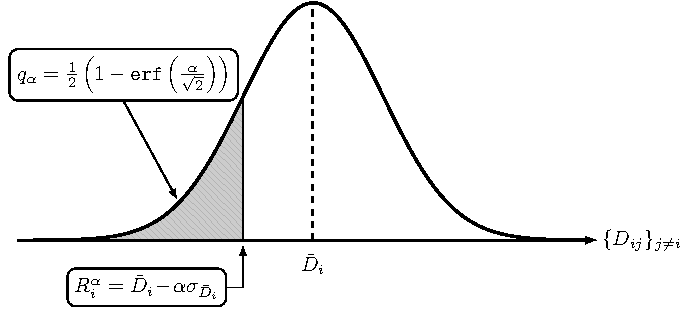
\includegraphics[width=0.95\textwidth]{shaded_bell_curve.pdf}}
\end{minipage}%\hspace{0.15cm}
\begin{minipage}[h]{0.3\textwidth}
\noindent\refstepcounter{figure}\textbf{Fig \thefigure \label{fig:gaussPlot}.} Illustration of the expected probability of a fixed instance $j$ being in the fixed radius neighborhood of another instance $i$. The fixed radius is parameterized by a fraction $\alpha$ of the standard deviation of all pairwise distances measured from instance $i$ to all possible neighbors.
\end{minipage}
\end{figure} 

\section{Data simulations}\label{sec:sim_methods}
In this section, we discuss our methods of generating interaction effects, main effects, and a combination of main and interaction effects. In our analysis of optimizing $k$, we use mixed simulations containing main and interaction effects to determine the best overall strategy of choosing $k$ for a given scenario on the data.

\subsection{Interaction effects}

We extend an interaction effect simulation method that generates differential correlation starting from a random graph from either Erd\H{o}s-R\'{e}nyi or Scale-free degree distribution~\cite{lareau15}. With this method, functional features in the control group are given large pairwise correlations with all other features. Differential correlations (interaction effects) are created by randomly permuting functional feature data entries within the case group only, which destroys the correlation structure in the case group but preserves the correlation structure in the control group. This method creates large effect sizes, which are easily detected by nearest-neighbor distance based methods. The reason for this ease of detection is the uniformity in low and high correlations in case and control groups, respectively. 

In order to establish more influence over the number of differential pairwise correlations, we simulate correlation matrices for case and control groups directly. We allowed only functional connections to be given differential correlation between case and control groups, where a functional connection is simply the presence of an edge (or link) from one feature to a functional feature in the random network that is generated. We show a flow diagram that displays our simulation method for interactions (Figure~\ref{fig:mixed_sim}). Analogous to the former method~\cite{lareau15}, we start with a random graph with either Erd\"{o}s-R\'{e}nyi or Scale-free degree distribution (Figure~\ref{fig:mixed_sim}\textbf{(1)}). From the random graph, we choose which attributes will be given functional interactions ($F$) among those with non-zero degree (Figure~\ref{fig:mixed_sim}\textbf{(2)}). Using adjacency matrix $A$, along with the indices of interaction attributes $F$, we create correlation matrices for cases and controls (Figure~\ref{fig:mixed_sim}\textbf{(3)}). For the control group, we assign high correlations ($\rho^\text{hi}$) to connected attribute pairs from the random graph while non-connected pairs are given low correlation ($\rho^\text{lo}$). We add noise ($\varepsilon_{ij} \sim \mathcal{N}(0,0.1)$) to the high and low correlation parameters as well, which gives each pair of attributes a different correlation. The case group starts out with the same exact correlation matrix as the controls ($P^\text{ctrl}$). For attributes that are connected to another attribute that is functional ($F$), we create differential correlation for these pairs using the parameter
\begin{equation}\label{eq:b_int}
b^\text{int} = - t \rho^\text{hi} + (1 - t) \rho^\text{hi}, \text{ where } t \in [0,1].
\end{equation}
As $t \to 0$, the effect size decreases monotonically. On the other hand, the effect size increases monotonically as $t \to 1$. By controlling $\rho^\text{hi}$, $b^\text{int}$, and the level of network connectivity, we have the ability to more finely control the interaction effect size than the preceding simulation method upon which ours is drawn~\cite{lareau15}. 

After correlation matrices are created for cases ($P^\text{case}$) and controls ($P^\text{ctrl}$), we compute the upper triangular Cholesky factors ($U^\text{case}$ and $U^\text{ctrl}$) for each correlation matrix (Figure~\ref{fig:mixed_sim}\textbf{(4)}). We then simulate null data matrices $X^\text{case}$ and $X^\text{ctrl}$  (Figure~\ref{fig:mixed_sim}\textbf{(5)}) for cases and controls, respectively, such that 
\begin{equation}\label{eq:null_case_ctrl}
x^\text{case}_{ij}, x^\text{ctrl}_{ij} \sim \mathcal{N}(0,1) \quad \forall i,j.
\end{equation}
Multiplication of $X^\text{case}$ and $X^\text{ctrl}$ by the Cholesky factors $U^\text{case}$ and $U^\text{ctrl}$, respectively, produce case and control sub-matrices $Y^\text{case}$ and $Y^\text{ctrl}$ with the correlation structure described previously. These sub-matrices are then combined into a single data $m \times p$ matrix given by
%
\begin{equation}\label{eq:full_interaction_data}
X^\text{int} = \left[
\begin{array}{c}
Y^\text{ctrl} \\ [0.5ex]
\hdashline \\ [-1.7ex]
Y^\text{case}
\end{array}
\right].
\end{equation}
%

The final interaction data set ($X^\text{int}$) contains both functional interacting attributes and noise attributes with no effect. We can use the interaction simulation algorithm (Figure~\ref{fig:mixed_sim}\textbf{(1)}\textbf{(5)}) to generate only interactions, or we can use the final step of the algorithm (Figure~\ref{fig:mixed_sim}\textbf{(5)}) in combination with main effect simulations to create data with mixed effects (Figure~\ref{fig:mixed_sim}\textbf{(6)}-\textbf{(7)}). We explain the main effect simulations (Figure~\ref{fig:mixed_sim}\textbf{(6)}) in the next section.

%\begin{figure}[H]
%\centering

% \framebox{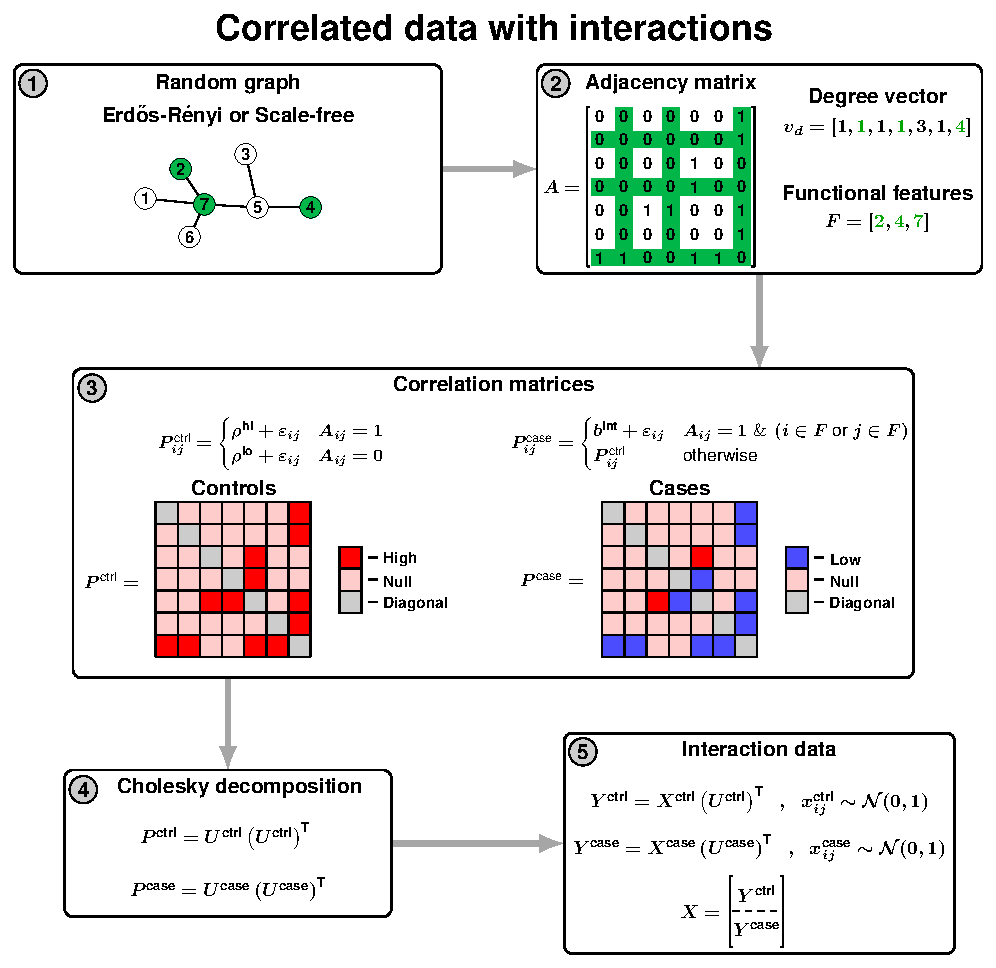
\includegraphics[width=0.98\textwidth]{interaction_simulation_method_diagram2.pdf}}
% \caption{Algorithm for interaction simulations from a random undirected network with seven nodes (or features). \textbf{Box 1:} A random network is generated, whose degree distribution is either Erd\H{o}s-R\'{e}nyi or Scale-free. \textbf{Box 2:} Adjacency matrix ($A$) and degree vector ($v_d$) corresponding to the random network are computed and functional features ($F$) are randomly selected from those with positive degree. \textbf{Box 3:} Two correlation matrices are generated for cases and controls. In the control group, high ($\rho^\text{hi}$) and low ($\rho^\text{lo}$) correlations are assigned to connected ($A_{ij}=1$) and non-connected ($A_{ij}=0$) feature pairs, respectively. In the case group, differential correlation ($b^\text{int}$) is applied to functional connections. \textbf{Box 4:} Upper triangular Cholesky factors are computed for case/control correlation matrices. \textbf{Box 5:} Standard normal random data matrices ($X^\text{ctrl}$ and $X^\text{case}$) are given correlation structure associated with case and control groups and combined into full data matrix with interaction effects ($X$).}\label{fig:interaction_simulation_diagram}
%\end{figure}


\subsection{Main effects}
We use a method for generating main effects that was previously applied to the study of gene expression data~\cite{leek2007}. This method uses a linear model given by
%
\begin{equation}\label{eq:lin-mod}
X_{ia} = b_a y_i + \varepsilon_{ia},
\end{equation}
%
where $b_a \sim \mathcal{N}(0,b^\text{main})$ for some fixed $b^\text{main}>0$, $y_i \in \{0 (\text{control}),1 (\text{case})\}$, and $\varepsilon_{ia} \sim \mathcal{N}(0,1)$. We show an illustration of this method (Figure~\ref{fig:mixed_sim}\textbf{(6)}), where the end result ($X^\text{main}$) contains three main effect attributes with effects sizes determined by $B^\text{T}=[b_1,b_2,b_3]$. The effect sizes vanish in the lower block of matrix $(BY)^\text{T}$ because this lower block represents the control group whose class labels are 0. The magnitude of $b^\text{main}>0$ determines the effect size between case and control groups. We add noise ($E$) so that case and control groups are both normally distributed with different means with respect to each main effect, but have approximately the equal variance.

\subsection{Mixed effects: interactions and main effects}
In order to simulate data with both interactions and main effects, we combine the interaction simulations (Figure~\ref{fig:mixed_sim}\textbf{(5)}) and main effect simulations (Figure~\ref{fig:mixed_sim}\textbf{(6)}) into a single data set ($X$) (Figure~\ref{fig:mixed_sim}\textbf{(7)}), where the left block matrix of $X$ contains interactions and noise and the right block of $X$ contains only main effects. Our mixed effects (interactions + main effects) simulation method can be used to create a wide variety of different types of data sets. In particular, our interaction simulation strategy is novel in that we simulate correlation matrices for cases and controls directly. We tune the interaction effect size by adjusting $\rho^\text{hi}$, $b^\text{int}$ (Eq.~\ref{eq:b_int}), and the degree of connectivity of interacting attributes in the random graph (Figure~\ref{fig:mixed_sim}\textbf{(1)}).

\begin{figure}[H]
 \centering
 \framebox{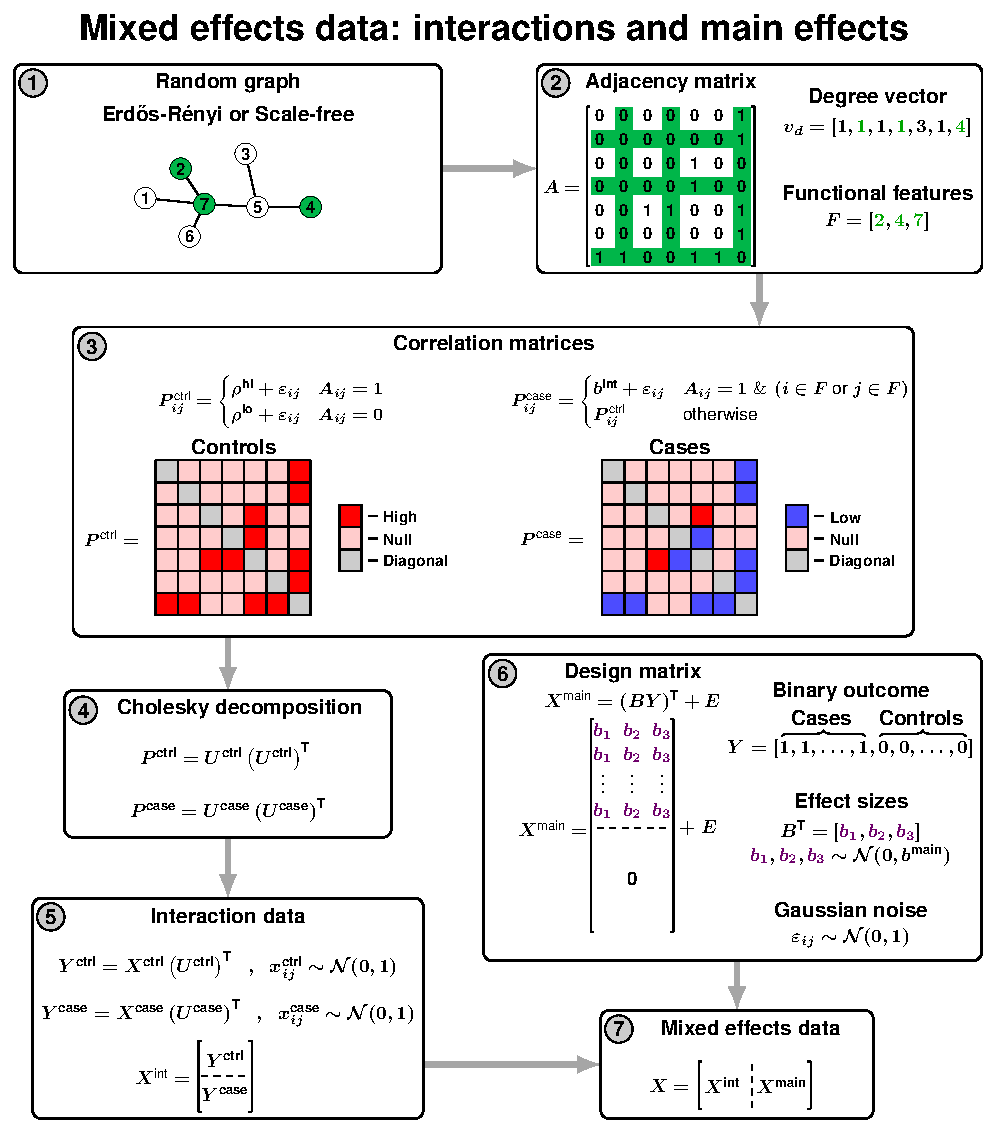
\includegraphics[width=0.9\textwidth]{mixed_simulation_diagram2.pdf}}	
 \caption{Algorithm for simulating mixed effects data with interactions and main effects. \textbf{(1)} Random network is generated, whose degree distribution is either Erd\H{o}s-R\'{e}nyi or Scale-free. \textbf{(2)} Adjacency matrix ($A$) and degree vector ($v_d$) corresponding to the random network are computed and functional features ($F$) are randomly selected from those with positive degree. \textbf{(3)} Correlation matrices are generated for cases and controls. In the control group, high ($\rho^\text{hi}$) and low ($\rho^\text{lo}$) correlations are assigned to connected ($A_{ij}=1$) and non-connected ($A_{ij}=0$) feature pairs, respectively. In the case group, differential correlation ($b^\text{int}$) is applied to functional connections. \textbf{(4)} Upper triangular Cholesky factors are computed for case/control correlation matrices. \textbf{(5)} Standard normal random data matrices ($X^\text{ctrl}$ and $X^\text{case}$) are given correlation structure associated with case and control groups and combined into full data matrix with interaction effects ($X$). \textbf{(6)} Main effects simulated with effect sizes randomly sampled from $\mathcal{N}(0,b^\text{main})$. \textbf{(8)} Interactions ($X^\text{int}$) and main effects ($X^\text{main}$) combined $X$.}\label{fig:mixed_sim}
\end{figure}

\section{Optimizing \texorpdfstring{$k$}{} for detecting effects}\label{sec:optim-k}

We use a method that we call Variable-Wise Optimized $k$ (VWOK), formerly referred to as Gene-wise Adaptive $k$ (GWAK)~\cite{mckinney13}, to determine the optimal $k$ for each attribute in a particular simulated data set (Figure~\ref{fig:vwok}). VWOK maximizes the scoring metric for each individual attribute, where we use standardized NPDR beta coefficients for scoring attributes in our analysis. The winning score is the one that maximizes the NPDR beta coefficient for each attribute. Winning scores are sorted from largest to smallest, along with the corresponding pseudo P values from NPDR, and those with significant adjusted P values are selected for further analysis. The VWOK method can be applied similarly using any nearest-neighbor feature selection algorithm, such as Relief-Based Algorithms~\cite{urbanowicz17}. The success of VWOK relies on the fact that scores of noise attributes do not change significantly as a function of $k$, while functional attribute scores do change significantly and have a well defined maximum with respect to $k$. Another reason we use VWOK is because we can explore all values of $k$, from $k=1$ to $k=m-1$, for each attribute.  

\begin{figure}[!hbt]
	\centering
	\framebox{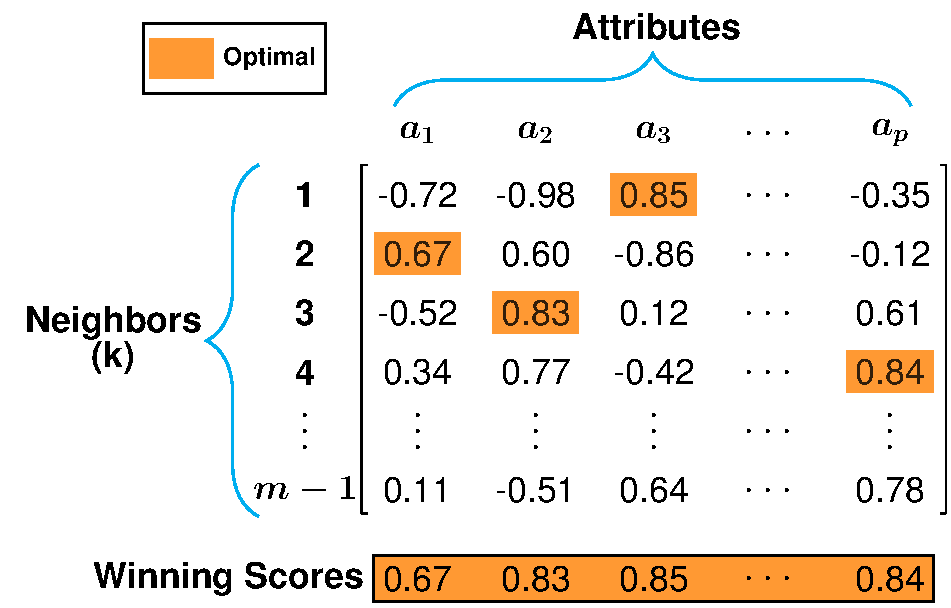
\includegraphics[width=0.65\textwidth]{feature_wise_opt_diagram3.pdf}}
	\caption{Variable-Wise Optimized $k$ (VWOK) method for choosing optimal values of $k$ in nearest-neighbor feature selection. For each attribute $a$ and each value of $k=1,2,\dots,m-1$, a score or weight is computed with a nearest-neighbor feature selection method like Relief-Based Algorithms (RBAs) or another similar method. Each feature is assigned the value of $k$ that maximizes its importance score. Winning scores are then sorted in decreasing order and some fraction of the top scoring attributes are chosen for further analysis. In our analysis, we use standardized NPDR beta coefficients to score attributes, where adjusted pseudo P values are used to filter out insignificant attributes.}\label{fig:vwok}
\end{figure}

The ability to detect main effects increases monotonically with increasing $k$, while detection of interactions is optimized for intermediate values of $k$. To explore this, we generated 30 data sets with main effects and 30 data sets with interactions, where each data set had $m=p=100$ instances and attributes. For each data set and each value of $k$, we computed standardized NPDR beta coefficients. We then computed the area under the Precision-Recall Curve (auPRC) for each set of beta coefficients. For each value of $k$, we plotted the average auPRC from the 30 simulation replicates for both main effects and interaction effects (Figure~\ref{fig:auPRC-vs-k}). We observed that auPRC for data sets with main effects increases monotonically with increasing $k$. For data with interaction effects, there is a more complicated relationship between auPRC and $k$. We see an increase in auPRC between $k=1$ and $k=18$, but then there is no significant change until after $k=38$. Between $k=39$ and $k=99$, auPRC for data with interactions decreases monotonically with increasing $k$. Such different detectability between interactions and main effects produces a dilemma for fixed $k$ and fixed radius methods. If neighborhood selection parameters are too large, then neighborhoods will be tuned for detecting main effects but too large to detect interactions. A similar result happens if neighborhoods are too small, except we lose the ability to detect both types of effects. Real data typically has both interactions and main effects, so we must consider the implications of a particular parameterization for nearest-neighbor feature selection algorithms. With VWOK, we can tune $k$ for each individual attribute to avoid having to choose between the different types of effects.

\begin{figure}[!bht]
	\centering
	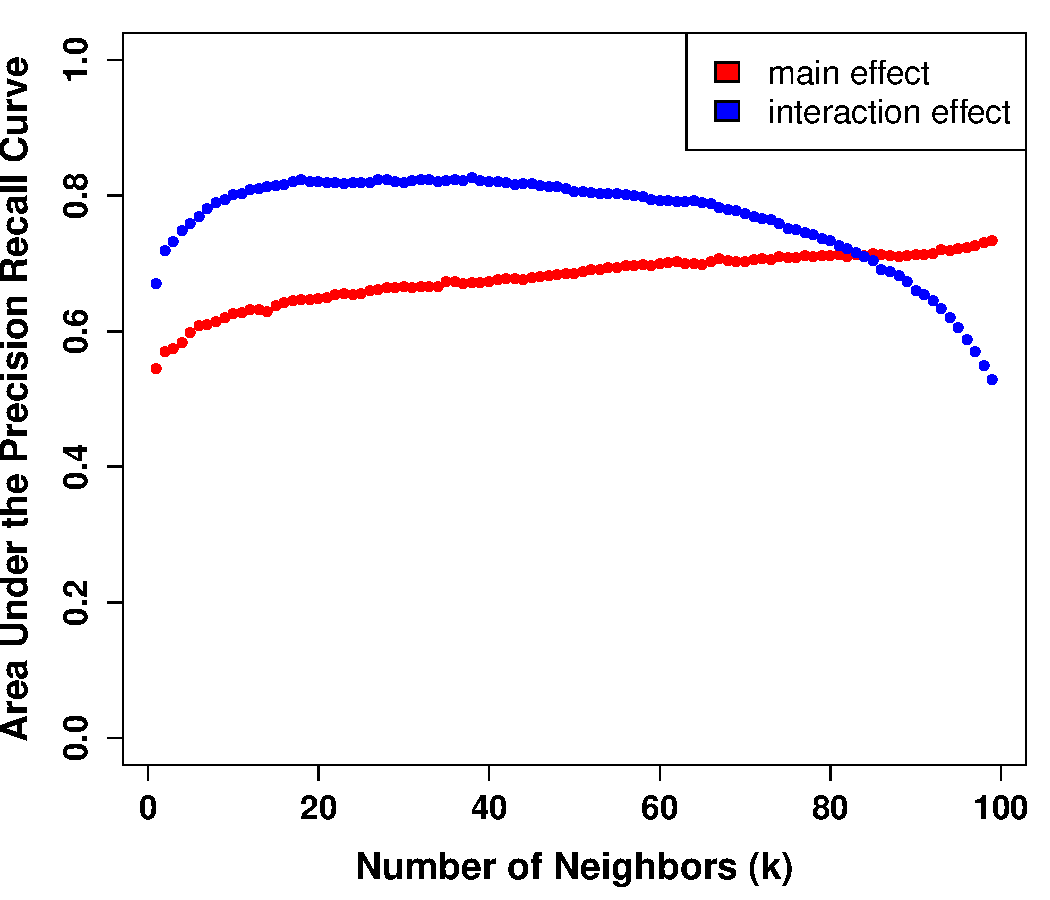
\includegraphics[width=0.8\textwidth]{auPRC_vs_k.pdf}
	\caption{Area Under the Precision-Recall Curve (auPRC) as a function of $k$ for simulated data. Each point on the plot is the average auPRC from 30 simulated data sets with interactions or main effects. Each data set has $m=p=100$ instances and attributes. Attribute scores were computed with NPDR~\cite{npdr2}. The auPRC monotonically increases with increasing $k$ and is maximized at $k=m-1=99$ for main effects. For interactions, auPRC increases between $k=1$ and $k=18$ and remains relatively constant until $k=38$. After $k=38$, auPRC decreases monotonically between $k=39$ and $k=99$.}\label{fig:auPRC-vs-k}
\end{figure}

%\vspace{0.2cm}

%{\centering
%	\begin{minipage}[c]{0.55\textwidth}
%		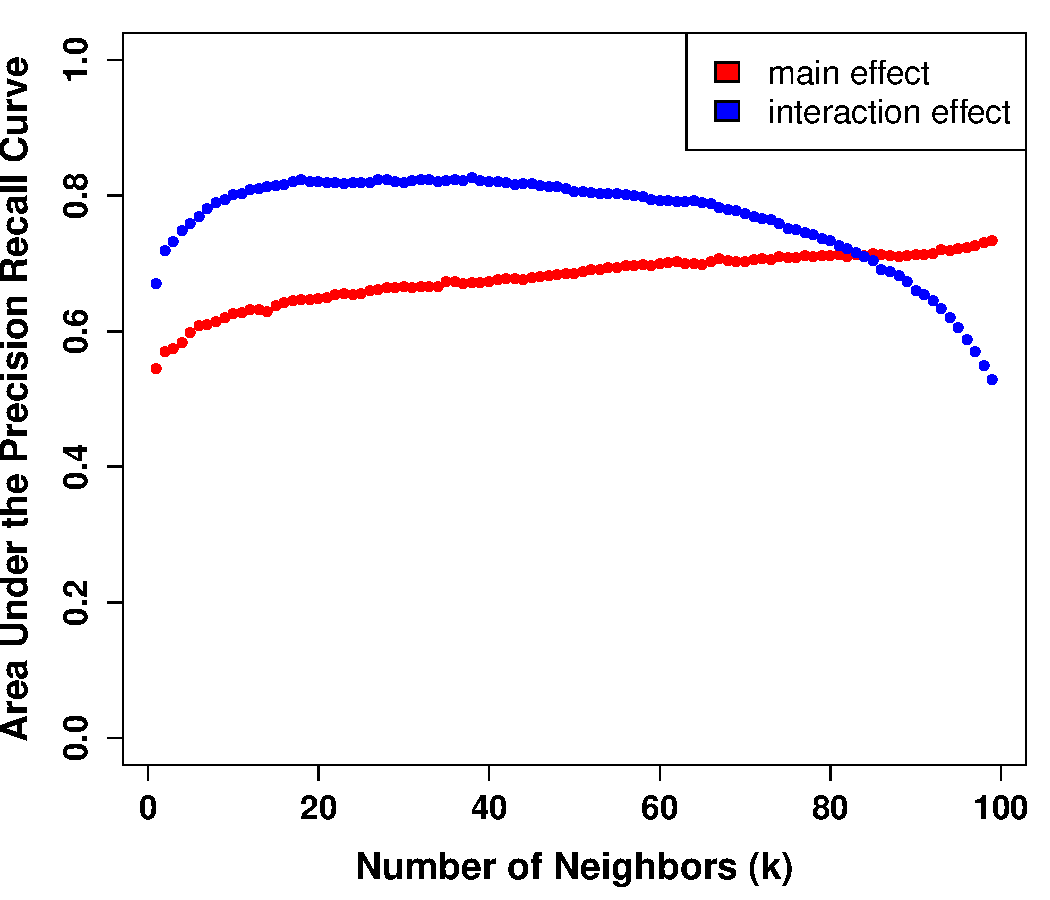
\includegraphics[width=1\textwidth,clip,trim=0cm 0cm 0cm 0.0cm]{auPRC_vs_k.pdf}
%	\end{minipage}\hfill
%	\begin{minipage}[c]{0.43\textwidth}
%		\captionsetup{type=figure}\captionof{figure}{Area Under the Precision-Recall Curve (auPRC) as a function of $k$ for simulated data. Each point on the plot is the average auPRC from 30 simulated data sets with interactions or main effects. Each data set has $m=p=100$ instances and attributes. Attribute scores were computed with NPDR~\cite{npdr}. The auPRC monotonically increases with increasing $k$ and is maximized at $k=m-1=99$ for main effects. For interactions, auPRC increases between $k=1$ and $k=18$ and remains relatively constant until $k=38$. After $k=38$, auPRC decreases nearly monotonically between $k=39$ and $k=99$.}\label{fig:auPRC-vs-k}
%\end{minipage}}

%\vspace{0.2cm}

Because our goal in this analysis is not necessarily model selection, but rather feature selection where we know which features are functionally related to the outcome, we apply VWOK without splitting the data into training and test folds. Generally, one would intuitively apply a cross-validation method, such as nested cross-validation (nested-CV), for parameter tuning to avoid overfitting (Figure~\ref{fig:nCV}). 

\begin{figure}[!bht]
	\centering
	\framebox{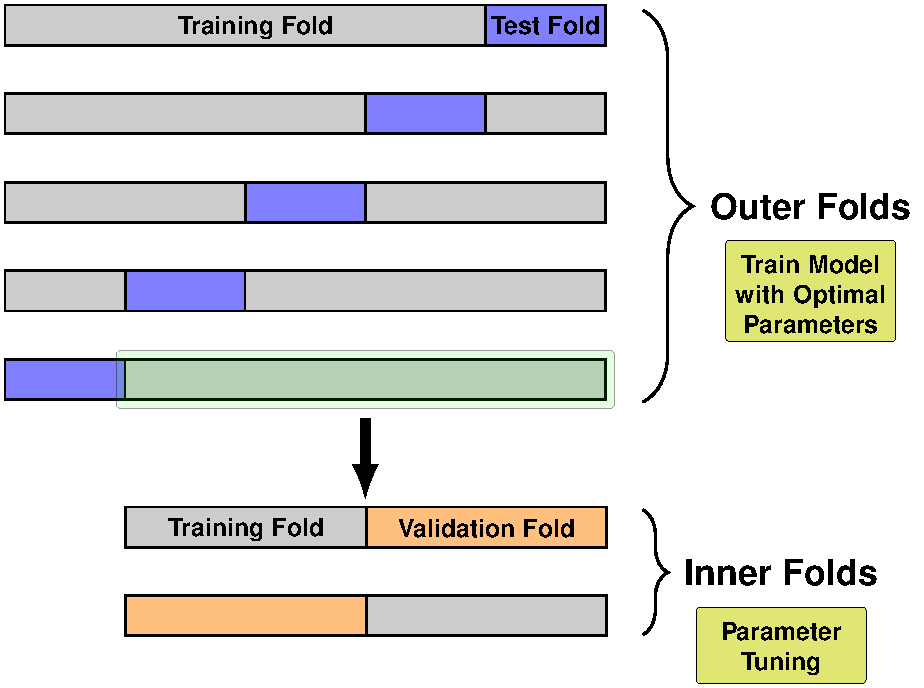
\includegraphics[width=0.7\textwidth]{nested_cv_diagram.pdf}}
	\caption{Nested cross-validation algorithm for simultaneously tuning parameters and selecting models. The data is split into training and test folds, where each outer training fold is further split into training and validation folds in order to tune parameters and select features. Parameters and features are chosen in the inner folds to optimize validation accuracy. Selected features and tuned parameters from the inner loop are used to train on the full outer training fold. Features and tuned parameters corresponding with the highest outer test accuracy are ultimately selected.}\label{fig:nCV}
\end{figure}

However, we have seen empirically that cross-validation does not produce high quality attributes in the context of nearest-neighbor feature selection. We compared the Area Under the Precision-Recall Curve (auPRC) for Global best fixed $k$, VWOK, and (nested-CV) on simulated data (Figure~\ref{fig:auPRC-compare-global-vwok-nCV}). Using our simulation method (Figure~\ref{fig:mixed_sim}), we generated 30 data sets with main effects and 30 data sets with interaction effects. The best auPRC was computed for each data set with respect to $k$ using each of these methods. For a given data set, Global best fixed $k$ simply loops through each possible value of $k$, computes attribute scores with a nearest-neighbor feature selection algorithm, and chooses the value of $k$ that maximizes auPRC. One reason that cross-validation does not perform well in nearest-neighbor feature selection algorithms is because it optimizes classification accuracy and does not optimize attribute scores. With nearest-neighbor feature selection, we have seen that cross-validation methods tend to produce highly predictive models composed of largely irrelevant attributes. Also, we have the advantage of knowing which attributes are functional in simulated data so our only concern is to determine which value of $k$ maximizes the scores of these attributes. Because noise attribute scores do not change significantly as a function of $k$ but functional attribute scores do, we maximize the probability of selecting these functional attributes among those at the top of the ranking with VWOK. 

\begin{figure}[!bht]
	\centering
	\begin{tikzpicture}
	\node at (0,0) {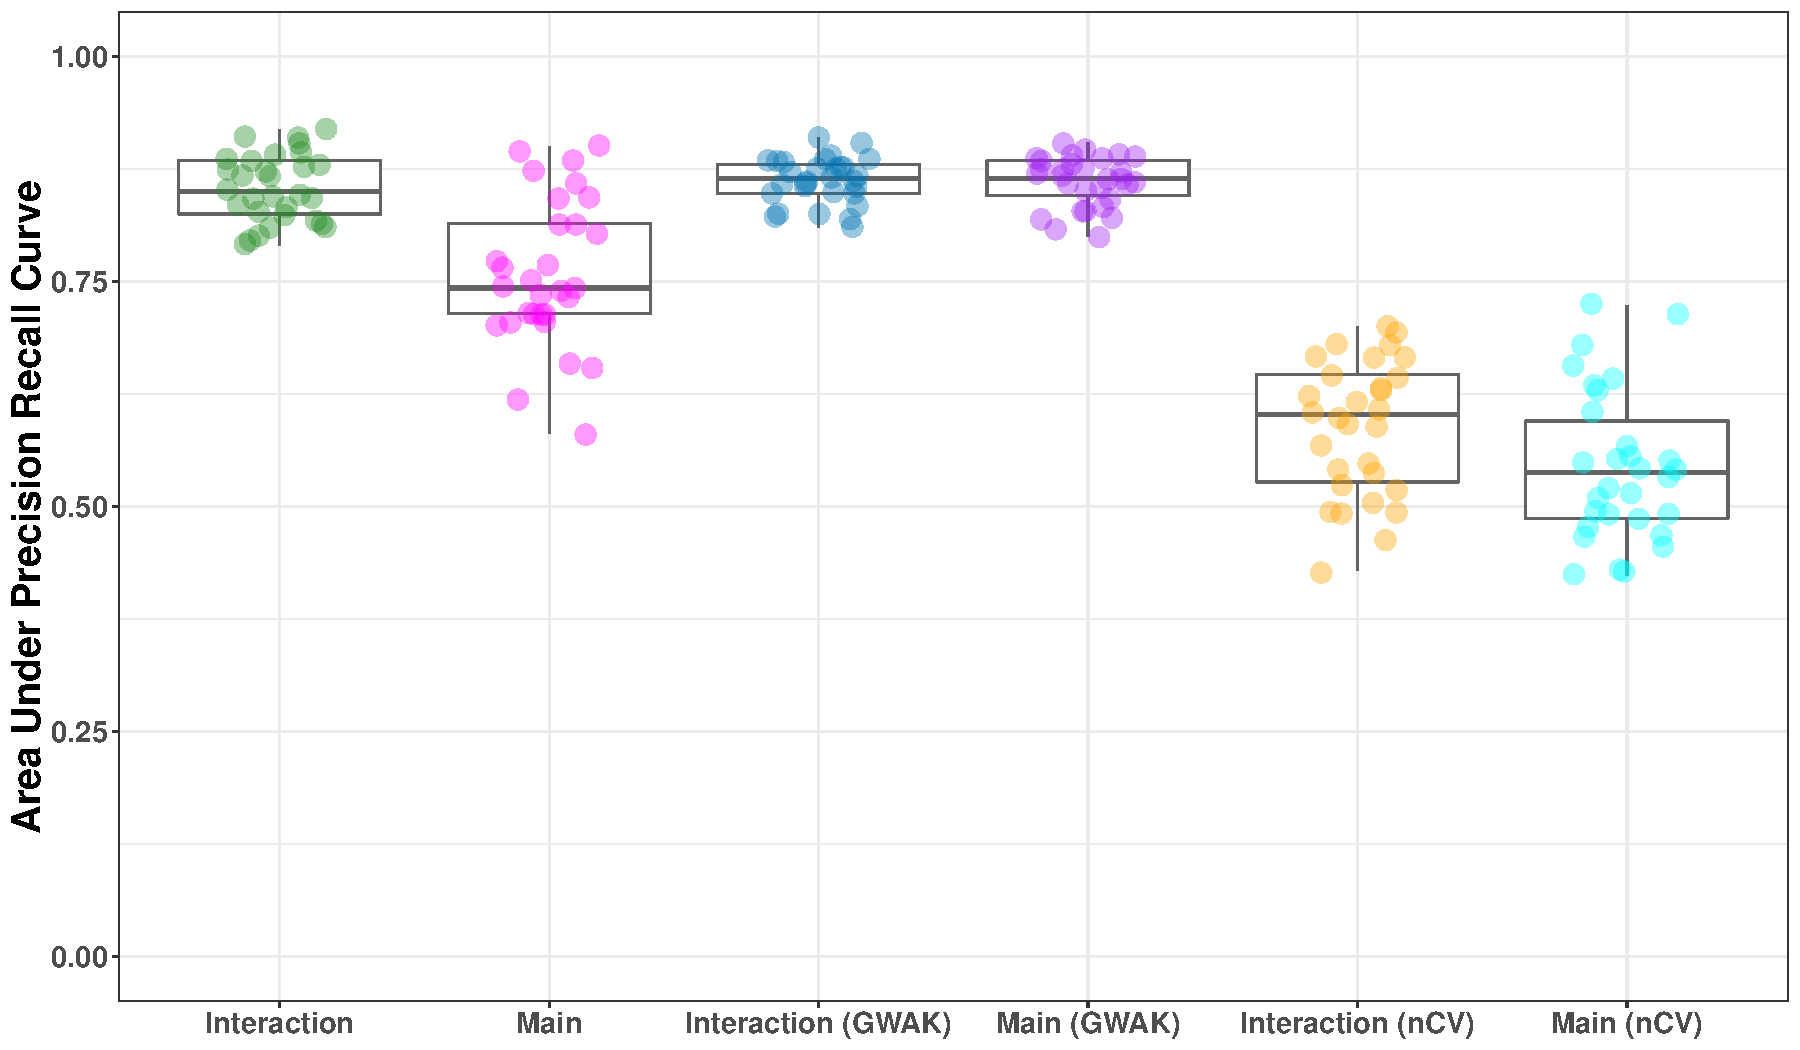
\includegraphics[clip,trim=0.2cm 0cm 0cm 0cm,width=0.98\textwidth]{global_best-k_auRC_vs_gwak_auRC_nestedCV_auRC.pdf}};
	
	\node[fill=white,xscale=0.8,yscale=0.8] at (-4.55,-3.73) {\textbf{Interaction}};
	\node[fill=white,xscale=0.8,yscale=0.8] at (-4.55,-4.1) {\textbf{(Global} \bm{$k$}\textbf{)}};
	
	\node[fill=white,xscale=0.8,yscale=0.8] at (-2.6,-3.73) {\textbf{Main}};
	\node[fill=white,xscale=0.8,yscale=0.8] at (-2.6,-4.1) {\textbf{(Global} \bm{$k$}\textbf{)}};
	
	\node[fill=white,text width=2cm,text height=0.2cm] at (-0.65,-3.73) {};
	\node[fill=white,xscale=0.8,yscale=0.8] at (-0.63,-3.73) {\textbf{Interaction}};
	\node[fill=white,xscale=0.8,yscale=0.8] at (-0.63,-4.1) {\textbf{(VWOK)}};
	
	\node[fill=white,text width=2cm,text height=0.2cm] at (1.3,-3.73) {};
	\node[fill=white,xscale=0.8,yscale=0.8] at (1.34,-3.73) {\textbf{Main}};
	\node[fill=white,xscale=0.8,yscale=0.8] at (1.34,-4.1) {\textbf{(VWOK)}};
	
	\node[fill=white,text width=2cm,text height=0.2cm] at (3.25,-3.73) {};
	\node[fill=white,xscale=0.8,yscale=0.8] at (3.32,-3.73) {\textbf{Interaction}};
	\node[fill=white,xscale=0.8,yscale=0.8] at (3.32,-4.1) {\textbf{(nested-CV)}};
	
	\node[fill=white,text width=2cm,text height=0.2cm] at (5.2,-3.73) {};
	\node[fill=white,xscale=0.8,yscale=0.8] at (5.3,-3.73) {\textbf{Main}};
	\node[fill=white,xscale=0.8,yscale=0.8] at (5.3,-4.1) {\textbf{(nested-CV)}};
	
	\node[fill=white,xscale=0.8,yscale=0.8,rotate=90] at (-6.45,0.15) {\textbf{Area Under Precision Recall Curve}};
	\end{tikzpicture}
	\caption{Comparison of Area Under the Precision-Recall Curve (auPRC) for three methods on simulated data with main effects or interactions. Each point on any particular boxplot represents the max auPRC for one of 30 simulated data sets, where auPRC is maximized as a function of $k$. We compared auPRC for each data set with respect to Global fixed $k$, Variable-Wise Optimized $k$ (VWOK), and nested cross-validation (nested-CV). VWOK has the best performance overall and the lowest variance in auPRC. Unlike the other methods, VWOK auPRC is balanced between interactions and main effects because each attribute has its own best $k$.}\label{fig:auPRC-compare-global-vwok-nCV}
\end{figure}

Using the same 30 simulated data sets with either interactions or main effects, we compared auPRC between VWOK, MultiSURF (MSURF), and MultiSURF average $k$ ($\bar{k}_\alpha$, Eq.~\ref{eq:kbar}) (Figure~\ref{fig:auPRC-compare-vwok-msurf-predk}). As in the comparison of VWOK with nested-CV and Global best $k$, we see that VWOK outperforms the other methods by consistently giving a higher auPRC on simulated data. The imbalance in interaction and main effect detection that is seen with MultiSURF vanishes with VWOK. The performances of adaptive radius MultiSURF and MultiSURF average $k$ ($\bar{k}_\alpha$, Eq.~\ref{eq:kbar}) are essentially the same. This provides further justification for using VWOK in nearest-neighbor feature selection algorithms.

\begin{figure}[!bht]
	\centering
	\begin{tikzpicture}
	\node at (0,0) {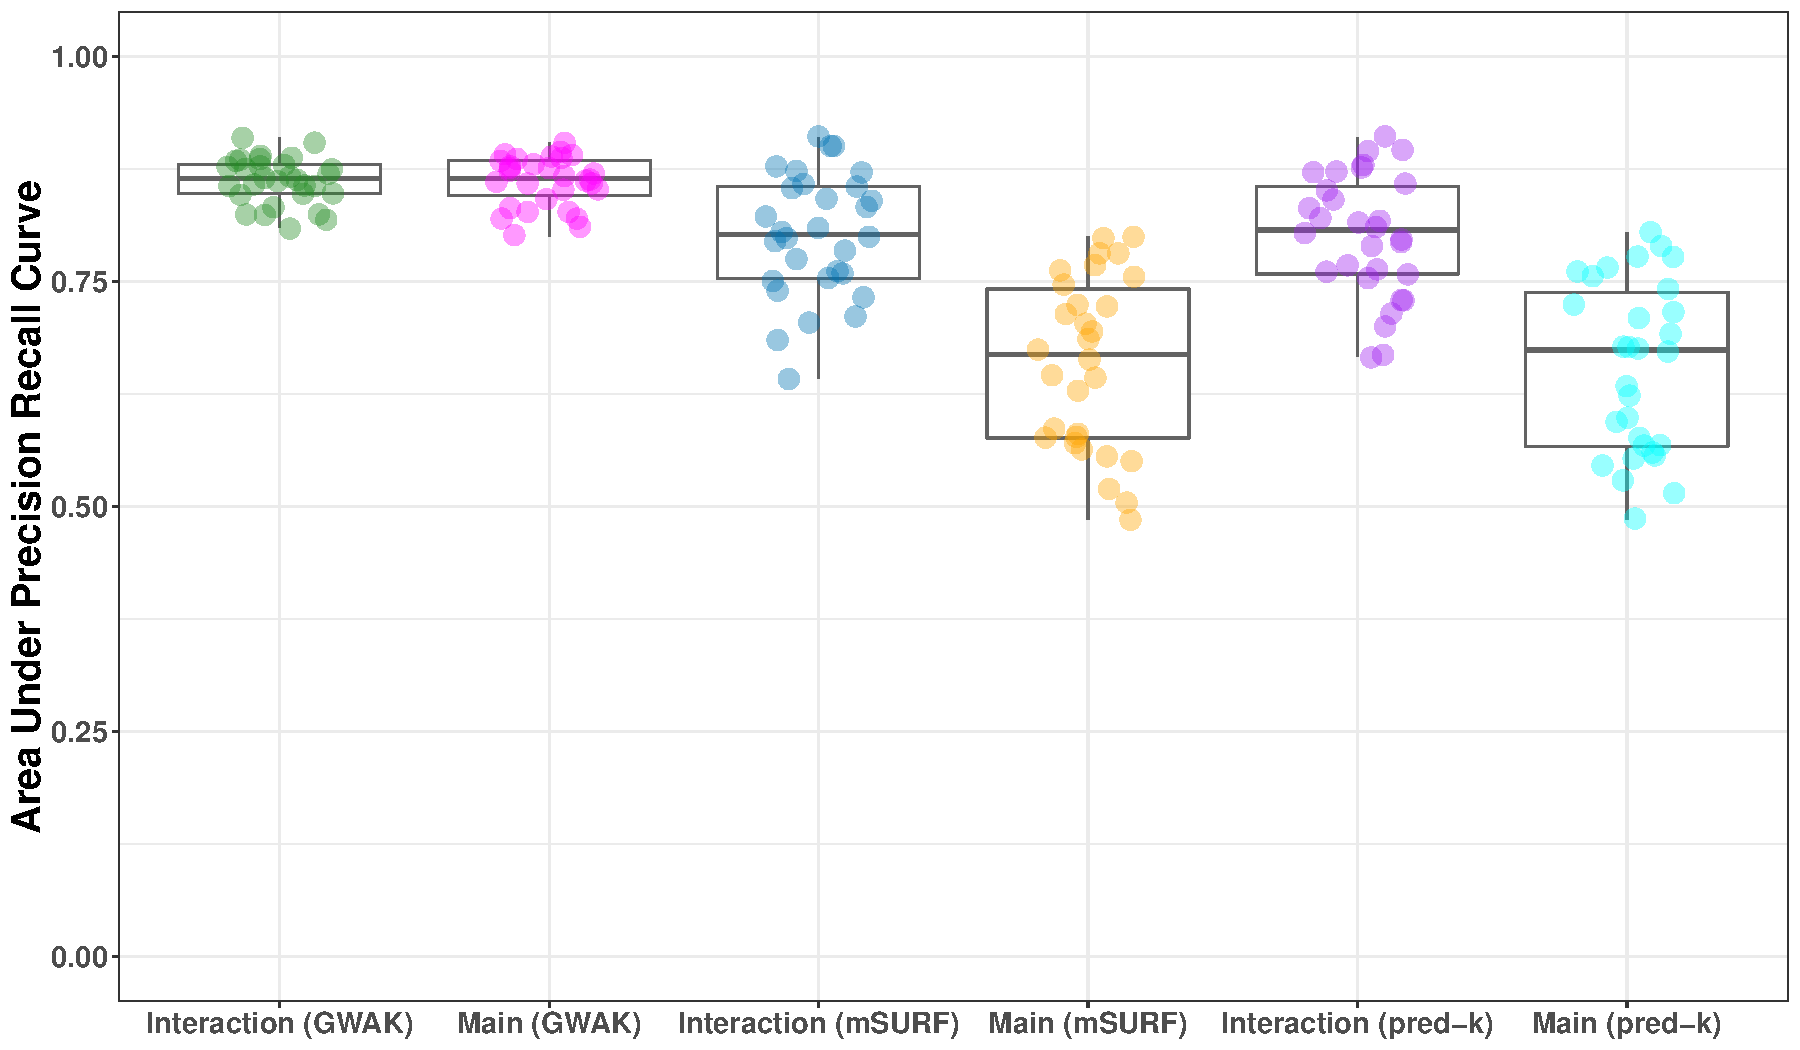
\includegraphics[clip,trim=0.2cm 0cm 0cm 0cm,width=0.98\textwidth]{gwak_auRC_vs_multisurf_auRC_vs_multisurf-predk_auRC.pdf}};
	
	\node[fill=white,text width=2cm,text height=0.2cm] at (-4.55,-3.73) {};
	\node[fill=white,xscale=0.8,yscale=0.8] at (-4.55,-3.73) {\textbf{Interaction}};
	\node[fill=white,xscale=0.8,yscale=0.8] at (-4.55,-4.1) {\textbf{(VWOK)}};
	
	\node[fill=white,text width=2cm,text height=0.2cm] at (-2.6,-3.73) {};
	\node[fill=white,xscale=0.8,yscale=0.8] at (-2.6,-3.73) {\textbf{Main}};
	\node[fill=white,xscale=0.8,yscale=0.8] at (-2.6,-4.1) {\textbf{(VWOK)}};
	
	\node[fill=white,text width=2cm,text height=0.2cm] at (-0.65,-3.73) {};
	\node[fill=white,xscale=0.8,yscale=0.8] at (-0.63,-3.73) {\textbf{Interaction}};
	\node[fill=white,xscale=0.8,yscale=0.8] at (-0.63,-4.1) {\textbf{(MSURF)}};
	
	\node[fill=white,text width=2cm,text height=0.2cm] at (1.3,-3.73) {};
	\node[fill=white,xscale=0.8,yscale=0.8] at (1.34,-3.73) {\textbf{Main}};
	\node[fill=white,xscale=0.8,yscale=0.8] at (1.34,-4.1) {\textbf{(MSURF)}};
	
	\node[fill=white,text width=2cm,text height=0.2cm] at (3.25,-3.73) {};
	\node[fill=white,xscale=0.8,yscale=0.8] at (3.32,-3.73) {\textbf{Interaction}};
	\node[fill=white,xscale=0.8,yscale=0.8] at (3.32,-4.1) {\textbf{(MSURF} \bm{$k$}\textbf{)}};
	
	\node[fill=white,text width=2cm,text height=0.2cm] at (5.2,-3.73) {};
	\node[fill=white,xscale=0.8,yscale=0.8] at (5.3,-3.73) {\textbf{Main}};
	\node[fill=white,xscale=0.8,yscale=0.8] at (5.3,-4.1) {\textbf{(MSURF} \bm{$k$}\textbf{)}};
	
	\node[fill=white,xscale=0.8,yscale=0.8,rotate=90] at (-6.45,0.15) {\textbf{Area Under Precision Recall Curve}};
	\end{tikzpicture}
	\caption{Comparison of Area Under the Precision-Recall Curve (auPRC) for three methods on simulated data with main effects or interactions. Each point on any particular boxplot represents the max auPRC for one of 30 simulated data sets, where auPRC is maximized as a function of $k$. We compared auPRC for each data set with respect to Variable-Wise Optimized $k$ (VWOK), adaptive radius method MultiSURF (MSURF), and predicted MultiSURF fixed $k$ (MSURF $k$). VWOK has the best performance overall and the lowest variance in auPRC. Unlike the other methods, VWOK auPRC is balanced between interactions and main effects because each attribute has its own best $k$.}\label{fig:auPRC-compare-vwok-msurf-predk}
\end{figure}

All simulation scripts for interactions, main effects, and mixed effects, were written in \textbf{\textsf{R}}~\cite{R}, and are available on Github (\url{https://github.com/insilico/npdr}). To explore how the optimal choice of $k$ changes in different contexts, we generated simulation replicates for several different scenarios on the data. Each simulated data set $X^{(m \times p)}$ generated contained $m=100$ instances and $p=1000$ features. We considered a balanced binary outcome only so that there were exactly $m/2$ cases and $m/2$ controls. In each simulation, 10\% of the total number of features $p$ were functionally related to the outcome variable while the remaining 90\% were simply background features with no effect. We also considered different ratios of main-to-interaction effect among functional attributes. Ratios of 0.2, 0.4, 0.6, and 0.8 of main-to-interaction, where 0.2 means that 20\% of the functional attributes are main effects while 80\% are interactions. For each simulation, we kept the main effect size parameter ($b^\text{main}$, Figure~\ref{fig:mixed_sim}\textbf{(6)}) fixed at 0.5 to reduce the total number of simulations. We explored different interaction effect sizes by varying the high correlation parameter ($\rho^\text{hi}$, Figure~\ref{fig:mixed_sim}\textbf{(3)}) only. The effect size increases monotonically with increasing $\rho^\text{hi}$ because $b^\text{int}$ is simply a point on the line from $-\rho^\text{hi}$ to $\rho^\text{hi}$, which is controlled by an input $t$ in our simulation \textbf{\textsf{R}} function. We considered values of $\rho^\text{hi} \in \{0.3,0.6,0.9\}$ so that we can explore small, medium, and large interaction effect sizes across all scenarios. The non-connection, low correlation parameter ($\rho^\text{lo}$, Figure~\ref{fig:mixed_sim}\textbf{(3)}) was fixed at 0.1 for all simulations. Taking all of the simulation parameters into account, we have a total of 12 different scenarios on data within our simulated data sets. For each scenario, we generate 30 replicates so that we can see the average value of fixed $k$ that optimizes functional attribute scores. We ran VWOK on each simulated data set to compute a value of $k$ for each attribute. Across all iterations for a given simulation scenario, the average VWOK value of $k$ that maximized the scores of interactions ($k^\text{int}_\text{ave}$), main effects ($k^\text{main}_\text{ave}$), and noise attributes ($k^\text{noise}_\text{ave}$) was computed. We also computed the average Global best $k$ ($k^\text{auPRC}_\text{ave}$), which is the average value of $k$ across all iterations of a given simulation scenario that maximized auPRC. For reasons we have already mentioned, we consider the VWOK values of $k$ to be the best choice for a given data set. Therefore, the average VWOK values of $k$ we computed are considered optimal for each simulation scenario. We give a summary from all of our simulation scenarios that shows the different values of $k$ for VWOK, Global best $k$, and MultiSURF (Table~\ref{tab:summary-k}). The VWOK average $k$ changes slightly for each type of attribute (e.g., main effects, interactions, and noise). The average VWOK $k$ for interactions ($k^\text{int}_\text{ave}$) is either 28 or 29, depending on different scenarios on the data. On the other hand, the average VWOK $k$ for main effects ($k^\text{main}_\text{ave}$) is either 58 or 61. There was no change in VWOK average $k$ for noise attributes ($k^\text{noise}_\text{ave}$), which remained fixed at 31 for each scenario. Interestingly, the average Global $k$ for optimizing auPRC ($k^\text{auPRC}_\text{ave}$) remained fixed at 27, which seems to favor interactions due to the similarity with the average VWOK $k$ for interaction effects ($k^\text{int}_\text{ave}$). For comparison, we computed the average MultiSURF neighborhood order ($k^\text{msurf}_\text{ave}$), which also remained fixed across each simulation scenario. The MultiSURF average $k$ is slightly larger than the corresponding VWOK average $k$, which could have implications for the ability of MultiSURF to optimally detect attributes. Skewness in the distance distribution, which is largely a result of high correlation simulation parameter ($\rho^\text{hi}$, Figure~\ref{fig:mixed_sim}), increases the probability of neighborhood inclusion ($q_\alpha$, Eq.~\ref{eq:q_prob}) slightly for MultiSURF. For any given target instance, this could lead to too many neighbors, which could reduce the ability to detect interactions as we have seen previously (Figure~\ref{fig:auPRC-vs-k}).

\begin{table}[H]
	\centering
	\caption{Summary of average fixed $k$ for three different methods. Using VWOK (Figure~\ref{fig:vwok}), we computed the average optimized $k$ for interactions ($k^\text{int}_\text{ave}$), main effects ($k^\text{int}_\text{ave}$), and noise attributes ($k^\text{noise}_\text{ave}$). We also applied Global best $k$ to optimize auPRC ($k^\text{auPRC}_\text{ave}$). The average MultiSURF $k$ ($k^\text{msurf}_\text{ave}$) is given for comparison. The high correlation parameter ($\rho^\text{hi}$, Fiure~\ref{fig:mixed_sim}\textbf{(3)}) was varied within $\{0.3,0.6,0.9\}$ to explore low, medium, and high correlation. Mix Ratio represents the ratio of main-to-interaction effects among functional attributes, where 0.2 means 20\% main effects and 80\% interactions.}\label{tab:summary-k}
	\begin{tabular}[h!]{ccccccc}\toprule
		\bm{$\rho^\textbf{hi}$} & \textbf{Mix Ratio} & \bm{$k^\text{int}_\text{ave}$} & \bm{$k^\text{main}_\text{ave}$} & \bm{$k^\text{noise}_\text{ave}$} & \bm{$k^\text{auPRC}_\text{ave}$} & \bm{$k^\text{msurf}_\text{ave}$} \\ \midrule
		0.3 & 0.2 & 28 & 61 & 31 & 27 & 32 \\
		0.3 & 0.4 & 28 & 61 & 31 & 27 & 32 \\
		0.3 & 0.6 & 28 & 61 & 31 & 27 & 32 \\
		0.3 & 0.8 & 28 & 61 & 31 & 27 & 32 \\
		0.6 & 0.2 & 29 & 58 & 31 & 27 & 32 \\
		0.6 & 0.4 & 29 & 58 & 31 & 27 & 32 \\
		0.6 & 0.6 & 29 & 58 & 31 & 27 & 32 \\
		0.6 & 0.8 & 29 & 58 & 31 & 27 & 32 \\
		0.9 & 0.2 & 28 & 61 & 31 & 27 & 32 \\
		0.9 & 0.4 & 28 & 61 & 31 & 27 & 32 \\
		0.9 & 0.6 & 28 & 61 & 31 & 27 & 32 \\
		0.9 & 0.8 & 28 & 61 & 31 & 27 & 32 \\ \bottomrule
	\end{tabular}
\end{table}

\section{Discussion}

In our analysis of optimizing the neighborhood selection parameter $k$ in nearest-neighbor feature selection algorithms, we have determined that there is no single value of $k$ that produces the best set of attributes from a given data set. The value of $k$ should adapt to each attribute in the data in order to maximize the ability to detect those that are relevant to a given outcome. 

\bibliographystyle{unsrt}
%\bibliography{BoD}   % name of bib file
\bibliography{BoD-rsfmri}
\end{document}
